\documentclass[pdf]{diss}
\usepackage[german,english]{babel}
\usepackage{setspace} 
\usepackage[refpage,intoc]{nomencl}
\usepackage[T1]{fontenc}
\usepackage{enumerate}
\usepackage{enumitem}
\usepackage{amsmath,amsthm,graphicx,amssymb,times,here} 
\usepackage{setspace}
\usepackage{multirow}
\usepackage{cite}
\usepackage{todonotes}
\usepackage[vlined,algoruled,linesnumbered,commentsnumbered]{algorithm2e}
\usepackage[export]{splitbib}
\usepackage[utf8]{inputenc}
\usepackage[tight,nice]{units}
\usepackage{xspace}
\usepackage{hhline}
\usepackage{todonotes}
\usepackage{booktabs}
\usepackage{here}
\usepackage{tikz}
\usepackage{rotating}
%\usepackage{subfigure}
\usepackage[caption=false]{subfig}
\setkomafont{captionlabel}{\sl}
\setkomafont{caption}{\sl}
\KOMAoption{captions}{centeredbeside}
%\usepackage{sidecap}
\setlength\pdfpagewidth{\paperwidth}
\setlength\pdfpageheight{\paperheight}
%\usepackage{hyperref}
\hypersetup{
	plainpages=false,
	hypertexnames=false,
	hidelinks
}

\newglossaryentry{N0}{
	name={\ensuremath{\mathbb{N}_0}},
	description={The set of positive integers including \(0\)}
}

\newglossaryentry{NodeB}{
	name={NodeB},
	description={Base station in an \acrshort{UMTS} mobile network}
}

\newglossaryentry{LTE}{
	name={LTE},
	description={Long Term Evolution. Fourth generation mobile communication standard developed by the \acrshort{3GPP}}
}

\newglossaryentry{TDCH}{
	name={\ensuremath{T_{\text{DCH}}}},
	description={Activity timer. \acrshort{UE} is demoted from \acrshort{RRC_DCH} state if no packets are sent or received for \ensuremath{T_{\text{DCH}}} seconds}
}

\newglossaryentry{TFACH}{
	name={\ensuremath{T_{\text{DCH}}}},
	description={Activity timer. \acrshort{UE} is demoted from \acrshort{RRC_FACH} state if no packets are sent or received for \ensuremath{T_{\text{FACH}}} seconds}
}


\newglossaryentry{RRCState}{
	name={\ensuremath{S}},
	description={Random variable describing the \acrshort{RRC} state of an \gls{UE}}
}

%TODO:
% - Random Variable A
% - Density Function of A
% - Distribution Function of A
% - Mean of A
% - Var of A

\newcommand{\specialcellbold}[2][c]{%
  \textbf{\begin{tabular}[#1]{@{}c@{}}#2\end{tabular}}}
	
	\newcommand{\specialcell}[2][c]{%
  \begin{tabular}[#1]{@{}c@{}}#2\end{tabular}}

\begin{category}{Bibliography of the Author}
	\begin{category}{Book Chapters}
		\SBentries{Zseby2011a}
	\end{category}
	\begin{category}{Journal Papers}
		\SBentries{Nguyen2013,Schwartz2013a,Hock2011}
	\end{category}
	\begin{category}{Conference Papers}		
	  \SBentries{Schwartz2014a,Hirth2014a,Burger2014a,Schwartz2013b,Schwartz2013c,Schwartz2012a,Hock2010a,Hock2010b,Hock2010c,Hartmann2009a}	
	\end{category}
	\begin{category}{Software Demonstrations}		
	\SBentries{Hock2011a}
	\end{category}	
\end{category}

\renewcommand{\SBmisctitle}{General References}
\SBtitlestyle{dash}
\SBsubtitlestyle{dash}

\topmargin-6.5mm
\textheight142mm

\renewcommand{\baselinestretch}{1.25}\normalsize

\newtheorem*{theorem}{Theorem}
\newtheorem*{corollary}{Corollary}

\let\oldbls=\baselinestretch
\newcommand{\leadingzero}[1]{\ifnum #1<10 0\the#1\else\the#1\fi}
\newcommand{\todayDK}{\leadingzero{\day}.\leadingzero{\month}.\the\year} 

%\date{\todayDK}
\date{xx.xx.2015}
\disputation{xx.xx.2015}
\serialnumber{3/15}
\issn{xxxx-xxxx}
\reviewer{Prof. Dr. Franco Davoli}
\place{Würzburg}

\author{Christian}{Schwartz}

\title{Modeling and Evaluation of Multi-Stakeholder Scenarios in Communication Networks}
 
%\preface{Danksagung}{danksagung}

\selectlanguage{english}
\AtBeginDocument{\renewcommand{\chapterautorefname}{Chapter}}
\AtBeginDocument{\renewcommand{\sectionautorefname}{Section}}
\AtBeginDocument{\renewcommand{\subsectionautorefname}{Section}}
\AtBeginDocument{\renewcommand{\subsubsectionautorefname}{Section}}
\AtBeginDocument{\newcommand{\subfigureautorefname}{Figure}}

\newcommand\alg[1]{Algorithm~\ref{alg:#1}}
\newcommand\fig[1]{Figure~\ref{fig:#1}}
\newcommand\figs[2]{Figures~\ref{fig:#1}--\ref{fig:#2}}
\newcommand\twofigs[2]{Figures~\ref{fig:#1} and \ref{fig:#2}}
\newcommand\sect[1]{Section~\ref{sec:#1}}
\newcommand\tabl[1]{Table~\ref{tab:#1}}
\newcommand\tables[2]{Tables~\ref{tab:#1} and \ref{tab:#2}}
\newcommand\reqn[1]{Equation~(\ref{eqn:#1})}

\begin{document}

\nocite{Nguyen2013,Schwartz2013a,Hock2011,Schwartz2014a,Hirth2014a,Burger2014a,Schwartz2013b,Schwartz2013c,Schwartz2012a,Hock2010a,Hock2010b,Hock2010c,Hartmann2009a,Hock2011a}

\setcounter{tocdepth}{4} 

\clearpage

\chapter{Introduction}\label{chap:introduction}

Todays internet is no longer controlled by few standard bodies, telecommunications companies and hardware vendors. 
New Internet applications are developed by start ups at an increasing rate, and each application has the potential to disrupt the status quo, both in business and technology.
These new applications not only impact the network infrastructure, but also a large set of Stakeholders participating in todays ecosystem of applications.

%\section{Considered Stakeholders}
\section{Scientific Contribution}
This monograph studies the interactions between different stakeholders in three, partially overlapping, scenarios in order to paint a broad picture of todays interlocking network and application ecosystem.

In \reffig{fig:introduction:publications}

\begin{figure}
\centering
\includegraphics{introduction/figures/publication}
\caption{Contribution of this work as a classification of the research studies conducted by the author}\label{fig:introduction:publications}
\end{figure}

First, 
\section{Outline of Thesis}
\chapter{Network}\label{chap:network}
This chapter studies trade-offs between multiple stakeholders in mobile networks.
These trade-offs have only appeared with the advent of smartphones.
With traditional cell phones, traffic in networks was largely dominated by voice traffic and to a smaller degree by text and signalling messages.
So called feature phones also introduced, together with new applications, new types of traffic.
Here, mostly web traffic and, to a lesser extend, traffic generated by applications was occuring.
However, applications were either proprietary and designed by phone vendors or did not find widespread adoption, so that the generated traffic was of note.
The introduction of smartphones resulted in an increased amount of applications, developed by a decentralized developer community.
With the application ecosystem no longer being under control of network operators, as in the case of voice or text messages, or hardware vendors, as with bundled applications in feature phones, centralized network management and end-to-end traffic engineering became difficult for network operators.

Each of the stakeholders involved in the mobile networking landscape is interested in optimizing the network, device, or application performance in its own interest.
To this end, each of the stakeholders can manipulate the parts of the network that it controls.
The network operator can change network configuration parameters in order to reduce signalling load in the network.
Smartphones may terminate data connections earlier, decreasing power consumption
Application developers can increase polling intervals in their application layer protocols in order to increase \gls{QoE}.	
However, each of the parameters the stakeholders can influence in order to optimize the metrics of their individual converns, also influences the complete system and thus all other metrics.

The contribution of this chapter is threefold.
\begin{enumerate*}
\item We provide an algorithm to key performance metrics for the considered stakeholders from traffic traces, and evaluate exemplary traces for a set of popular applications.
\item We develop an analytic model in order to analyse theoretical and empirical distributions and derive the metrics of interest for the stakeholders.
\item We study the impact of network timer optimisation, a practice where network operators modify network parameters in order to optimise signalling load, on a involved stakeholders.
\end{enumerate*}

The content of this chapter is taken from~\cite{Schwartz2013a,Schwartz2013c}.
Its remainder is structured as follows.
First, we give a background of mobile networks and survey the relevant related work in \refsec{sec:network:background}.
We perform application traffic measurements and investigate the impact of application traffic on \gls{UE} power consumption, network signalling and web \gls{QoE} for a selected set of applications in \refsec{sec:network:network_traces}.
Then, we generalize our results by introducing an analytic model in order to derive metrics for state transition frequency and power consumption from arbitrary traffic distributions in \refsec{sec:network:performance_model}.
Finally, we conclude this chapter with lessons learned in \refsec{sec:network:lessons_learned}.

\section{Background and Related Work}\label{sec:network:background}

\subsection{\headershortacr{UMTS} Networks and the \headershortacr{RRC} Protocol}\label{sec:network:background:umts_rrc}
A \gls{3G} \gls{UMTS} mobile network consists of three main components, which are depicted in \reffig{fig:network:background:mobile_network_overview}: The \gls{UE}, the \gls{RAN}, and the \gls{CN}.
The \gls{RAN} is used to establish connectivity between the \gls{UE} and the \gls{CN}, which in turn can establish connectivity to the Internet, if required.

\begin{figure}
	\centering
	\includegraphics{network/background/figures/mobile_network_overview}
	\caption{Overview of Mobile Network}
	\label{fig:network:background:mobile_network_overview}
\end{figure}

\gls{UE} consists of devices used by end users, i.e. smartphones, tablets or data card enabled notebooks, but can also include \gls{M2M} devices.
The \gls{RAN} is, amongst other tasks, responsible for \gls{RRC}, packet scheduling and handover control.
It includes network entities such as the \gls{NodeB} and the \gls{RNC}.
The \gls{CN} provides the backbone network of the \gls{UMTS} network and provides connectivity to the Internet and the \gls{PSTN}.
Furthermore, functionality such as billing, authentication and location management is provided by the \gls{CN}.

In UMTS networks, the radio resources in the RAN between base station and UE are controlled and managed by the \gls{RRC} protocol~\cite{3GPP_RRC_Spec}.
The protocol offers services such as broadcast of network information, maintenance of a connection between the \gls{UE} and \gls{RAN}, establishment of point-to-point radio bearers for data transmission, \gls{QoS} control, and reporting and cell selection management.
The protocol is divided into different parts: services for upper layers, communication with lower layers, protocol states, \gls{RRC} procedures, and error control.
In particular, \gls{RRC} also participates in the co-ordination of other resource management operations such as channel measurements and handovers.
All \gls{RRC} procedures rely on protocol states which are defined to trigger action should be applied and which information must be signaled. 
The state are defined per \gls{UE} and for the connection between the \gls{UE} and the \gls{NodeB} station.
Typically there are five \gls{RRC} states characterizing a connection between \gls{UE} and \gls{NodeB}: \gls{idle}, \gls{URAPCH}, \gls{CELLPCH}, \gls{DCH}, and \gls{FACH}.
Whether a specific \gls{RRC} state is used in a specific mobile network depends on the configuration of the network by the provider.
In the following we concentrate on the most commonly observed~\cite{Qian2010} \gls{RRC} states \gls{idle}, \gls{DCH}, and \gls{FACH}.

\subsection{Measurements of \headershortacr{RRC} Parameters and Optimisation of Resource Consumption}\label{sec:network:background:measurement_optimisation}

\subsection{Smartphone Energy Consumption and \headershortacr{QoE}}\label{sec:network:background:energy_consumption_qoe}

\section{Inferring Signalling Frequency and Power Consumption from Network Traces}\label{sec:network:network_traces}
\subsection{Inferring State Transitions and Deriving Metrics}\label{sec:network:network_traces:performance_evaluation}
\gls{RRC} state transitions are triggered by the \gls{UE}’s firmware.
While solutions exist to capture RRC state transitions on specific hardware~\cite{zayas2010} they are not available for all modern smartphone platforms.
Other options to measure the required information include using costly hardware and use specific \glspl{UE}, usually not available to researchers and application developers.
This prevents the developers from evaluating the effect of their applications on the overall health
of the network.
Consequently, they can not take measures to prevent the harmful behaviour of their applications.
However, it is possible to infer the \gls{RRC} state transitions for a given packet trace if the network configuration is known.

First, we describe the setup used to capture network packet traces for arbitrary apps.
Then, we give an algorithm to infer the \gls{RRC} state transitions for a given packet trace.
Based on these state transitions, we can calculate the number of signalling messages generated
by the packet trace. 
Finally, we use the information on when which \gls{RRC} state was entered to calculate the power drain of the \gls{UE}’s radio interface.

\subsubsection*{Measurement Procedure and Setup}\label{sec:network:network_traces:performance_evaluation:measurement}
To investigate the behaviour of the application under study, we capture traffic during a typical use of the application on a \emph{Samsung Galaxy SII} smartphone.
The smartphone runs the Android operating system and is connected to the \gls{3G} network of a major German network operator.
To obtain the network packet traces we use the \texttt{tcpdump} application.
This application requires \emph{root} privileges which are obtained by rooting the device and installing the custom \emph{cyanogenmod} ROM \footnote{http://www.cyanogenmod.org}.
Once \texttt{tcpdump} is installed and running, we start the application under study and capture packet traces while the application is running.
Then, the \emph{android debugging bridge} is used to copy the traces to a workstation.
The traces contain \gls{IP} packets embedded in Linux Cooked Captures.
We require the \gls{IP} packets, thus we extracted the \gls{IP} packets which are used during the following analysis.

\subsubsection*{Inferring Network State}\label{sec:network:network_traces:performance_evaluation:inferring_network_state}
In this section we study the influence of the application traffic on \gls{RRC} state transitions and signalling messages.
Since \gls{RRC} state transitions can not be captured using commonly available tools, we introduce an algorithm to infer \gls{RRC} state transitions from \gls{IP} packet traces.
Using this algorithm we analyse the \gls{RRC} state transition frequency and signalling message load for the Two State Model and Three State Model.

Traffic below the network layer can not be measured without specific equipment which interfaces with the proprietary firmware of the \gls{UE} and is often out of reach for developers interested in assessing the impact of their applications on the network.
Based on the Two State and Three State models introduced in \refsec{sec:network:background:umts_rrc}, we process \texttt{tcpdump} captures of the application traffic.
However, it should be noted that this method is not restricted to a specific network model, but can be extended to any other network model as well.
Using these captures, we extract the timestamps when \gls{IP} packets are sent or received.
Furthermore, we require the timer values of the transition from \gls{RRC_DCH} state to \gls{RRC_FACH} state, \gls{TDCH}, and the timer for the transition between \gls{RRC_FACH} and \gls{RRC_idle} states, \gls{TFACH}.
Based on these informations \refalg{alg:network:network_traces:performance_evaluation:inferring_network_state:inference_algorithm} infers the timestamps of state transitions according to the \gls{3GPP} specification \cite{3GPP_RRC_Spec} for the Three State Model.
This algorithm can be simplified to also work for the Two State Model. 
Alternatively, a method to post process the results of the algorithm to obtain results for the Two State Model is given at the end of this section.
The algorithm first computes the inter-arrival times of all packets.
Then, each timestamp is considered.
If the \gls{UE} is currently in \gls{RRC_idle} state, a state transition to \gls{RRC_DCH} occurs at the moment the packet is sent or received.
If the inter-arrival time exceeds the \gls{TDCH} timer the \gls{UE} transitions to \gls{RRC_FACH} \gls{TDCH} seconds after the packet was sent or received.
Similarly, if the inter-arrival time exceeds both the \gls{TDCH} and \gls{TFACH} timers a state transition to \gls{RRC_idle} occurs \gls{TDCH} seconds after the state transition to \gls{RRC_FACH}.

\begin{algorithm}
  \begin{algorithmic}
    \Require{Packet arrival timestamps \emph{ts}\\
    \gls{RRC_DCH} to \gls{RRC_FACH} timer \gls{TDCH}\\
    \gls{RRC_FACH} to \gls{RRC_idle} timer \gls{TFACH}}
    \Ensure{Times of state transition \emph{state\_time}\\
    New states after state transitions \emph{state}}
    \State \texttt{interarrival(i)} $\leftarrow$ \emph{ts}(i+1) - \emph{ts}(i)
    \State \texttt{index} $\leftarrow 0$
    \ForAll{ts(i)}
      \If{\texttt{state(index)} = \gls{RRC_idle}}
        \State \texttt{index} $\leftarrow$ \texttt{index} + 1
        \State \texttt{state(index)} $\leftarrow$ \gls{RRC_DCH}
        \State \texttt{state\_time(index)} $\leftarrow$ ts(i)
      \EndIf
      \If{\texttt{interarrival}(i-1) $> \gls{TDCH}$}
        \State \texttt{index} $\leftarrow$ \texttt{index} + 1
        \State \texttt{state(index)} $\leftarrow$ \gls{RRC_FACH}
        \State \texttt{state\_time(index)} $\leftarrow$ ts(i) $+ \gls{TDCH}$
      \EndIf
      \If{\texttt{interarrival}(i-1) $> \gls{TDCH} + \gls{TFACH}$}
        \State \texttt{index} $\leftarrow$ \texttt{index} + 1
        \State \texttt{state(index)} $\leftarrow$ \gls{RRC_idle}
        \State \texttt{state\_time(index)} $\leftarrow$ ts(i) $+ \gls{TDCH} + \gls{TFACH}$
      \EndIf
    \EndFor
  \end{algorithmic}
  \caption{Inferring \headershortacr{RRC} state transitions based on \headershortacr{IP} timestamps}
  \label{alg:network:network_traces:performance_evaluation:inferring_network_state:inference_algorithm}
\end{algorithm}

\gls{UE} vendors always search for ways to decrease power drain of their devices.
A straightforward way to achieve this, if only the wellbeing of the \gls{UE} is considered, is to transition from \gls{RRC_DCH} state to \gls{RRC_idle} as soon as no additional data is ready for sending.
While this transition is not directly available in the 3GPP specification for the \gls{RRC} protocol \cite{3GPP_RRC_Spec}, a \gls{UE} may reset the connection, effectively transitioning from any state to \gls{RRC_idle}.
This behaviour can be modelled using the Two State Model introduced in \refsec{sec:network:background:umts_rrc}.

State transitions for the Two State Model can be calculated using a similar algorithm.
Alternatively, the behaviour of the Two State Model can be emulated using \refalg{alg:network:network_traces:performance_evaluation:inferring_network_state:inference_algorithm} if \gls{TFACH} is set to \SI{0}{\second} and all state transitions to \gls{RRC_FACH} are removed in a post processing step.

\subsubsection*{Calculating Signalling Frequency and Power Consumption}\label{sec:network:network_traces:calculating_metrics}

\begin{table}
\centering
  \caption{Number of signalling messages per \headershortacr{RRC} state transition perceived at the \headershortacr{RNC} (Taken From \cite{3GPP_RRC_Spec})}
  \label{tab:network:network_traces:calculating_metrics:signalling_messages}
\begin{tabular}{cccc}
	\toprule
    from/to & \gls{RRC_idle} & \gls{RRC_FACH} & \gls{RRC_DCH}\\
    \midrule
    \gls{RRC_idle} & -- & 28 & 32\\
    \gls{RRC_FACH} & 22 & -- & 6\\
    \gls{RRC_DCH} & 25 & 5 & --\\
    \bottomrule    
	\end{tabular}
\end{table}

In reality, the number of state transitions is not the metric of most importance if network signalling is to be evaluated.
Each state transition results in a number of \gls{RRC} messages between the \gls{UE} and different network components.
For this study we consider the number of messages observed at the \gls{RNC}, which can be found in \cite{3GPP_RRC_Spec} and is summarized in \reftab{tab:network:network_traces:calculating_metrics:signalling_messages}.
It can be seen that transitions from or to the \gls{RRC_idle} state are especially expensive in terms of number of messages sent or received.
This is due to the fact that upon entering or leaving the \gls{RRC_idle} state, authentication has to be performed. 
Note that for the Two State Model only transitions from or to the \gls{RRC_idle} state occur.
This results in the fact that for the same network packet trace the number of signalling messages occurring in the Two State Model is generally higher than in the Three State Model.
To obtain the total number of signalling messages, we weight the number of state transitions with the number of messages sent per state transitions.
Then, we average the number of state transitions over the measurement duration to obtain a metric for the signalling load at the \gls{RNC}, i.e. the \gls{SF}.
The inference algorithm does not differentiate between state changes caused by upstream or downstream traffic.
State changes caused by downstream traffic usually generate some additional signalling messages, as paging is involved.
The inference algorithm can be easily enhanced to support this behaviour.
However, the results discussed in the next section would only change quantitatively.
Furthermore, the algorithm can be easily adapted to new networking models or signalling numbers.

\begin{table}
  \centering
  \caption{Power consumption of the \headershortacr{UE} radio interface depending on current \headershortacr{RRC} state (taken from \cite{Qian2011a})}
  \label{tab:network:network_traces:calculating_metrics:power_consumption}  
  \begin{tabular}{cc}
  	\toprule
    \gls{RRC} State & Power Consumption\\
    \midrule
    \gls{RRC_idle} & \SI{0}{\milli\watt}\\
    \gls{RRC_FACH} & \SI{650}{\milli\watt}\\
    \gls{RRC_DCH} & \SI{800}{\milli\watt}\\
    \bottomrule
  \end{tabular}
\end{table}

From a users point of view, the signalling message frequency is of little importantance.
The user is interested in a low power drain as this increases the battery life of the device.
To calculate the battery life, we use the time when state transitions occurred, and the information about the state the transition was to, to calculate the relative amount of time that was spent in each state.
Given the relative time spent in each state, we use \reftab{tab:network:network_traces:calculating_metrics:power_consumption}, taken from \cite{Qian2011a}, to compute the \gls{PD} of the radio interface during the measurement phase.
We focus on the power drain of the radio interface, as it is possible to measure the aggregated power drain using out of the box instrumentation techniques provided by the hardware vendor.
\subsection{Impact of Application Traffic Patterns}\label{sec:network:network_traces:numerical_results}
In the measurement study, we apply the methods introduced in \refsec{sec:network:network_traces:performance_evaluation} to four popular smartphone
applications to infer signalling traffic and power drain.
First, we characterize the applications in terms of traffic patterns, application usage, as well as bandwidth requirements.
Then, we study the \gls{SF} and power drain caused by these applications if inactivity timers, i.e. \gls{TDCH} or \gls{TFACH} are modified.
Finally, we analyse the influence of network parameters on web \gls{QoE} in terms of \gls{MOS} depending on page load times which are influenced by the network settings.

\subsubsection*{Characterization of Traffic Patterns for Selected Applications}\label{sec:network:network_traces:numerical_results:traffic_characterization}

\begin{table}
  \centering
  \caption{Qualitative characterization of applications under study}
  \label{tab:network:network_traces:numerical_results:app_characterization}
  \begin{tabular}{cccc}
  	\bottomrule
    Application&Traffic&Application&Required\\
    &Characteristic&Use&Bandwidth\\
    \midrule
    Angry Birds & Interactive & Foreground & Low bandwidth \\
    Aupeo & Interactive & Background & High bandwidth\\
    Twitter & Periodic, Low frequency & Background & Low bandwidth\\
    Skype & Periodic, High frequency& Background & Low bandwidth\\
    \bottomrule
  \end{tabular}
\end{table}

For this study we chose four specific applications in order to cover a broad spectrum of traffic characteristics, as described in \reftab{tab:network:network_traces:numerical_results:app_characterization}.
First, we discuss said characteristics for these applications.
We differentiate between applications, where the user interaction causes the generation of traffic, and such, where the application periodically sends or receives traffic.
Finally, we consider the amount of bandwidth used by the application.

\textbf{Angry Birds} for Android is a popular \emph{interactive} free-to-play game and runs in the \emph{foreground}.
To finance the game, an advertisement is shown once the player starts or restarts a level.
Advertisements are downloaded on demand by the application, but require \emph{low bandwidth}.
Thus, the time between two advertisements depends on the frequency of the player advancing to the next level or deciding to restart the current one.

\textbf{Aupeo} is an Internet radio application, allowing a user to listen to content from personalised radio stations, while running in the \emph{background}.
Content is not streamed but downloaded at the beginning of the track.
The exact duration depends on the radio stations chosen by the user and is thus \emph{interactive}.
This results in large times of inactivity during the playback of the track itself.
Due to the fact that audio files are downloaded, there is a \emph{high bandwidth} requirement.

The \textbf{Twitter} client is used to send and receive new short messages from the user's Twitter account.
Transferring these messages requires relatively \emph{low bandwidth}.
To this end, the user can specify an update frequency when to pull new messages in the \emph{background}.
Thus, the downloads occur with a \emph{periodic behaviour of low frequency}, where
the client sends an \gls{HTTPS} request to the Twitter server and in return receives new Tweets for the user's account.
We do not consider an active user who is publishing new Tweets.
Such behaviour would manifest as additional traffic to the periodic one generated by the status updates.
Due to the fact that publishing updates occurs relatively infrequent, and updating the feed occurs more often, the traffic generated by publishing updates is dominated by that occurring due to updates, and thus can be neglected.

Finally, we consider the \textbf{Skype} application.
We do not consider any \gls{VoIP} calls, but the application's idle behaviour, i.e. when the application is running in the \emph{background}.
During this time, the application sends keep-alive messages to the network.
These keep-alive messages are sent with a \emph{high frequency} and require \emph{low bandwidth}.

In addition to the applications considered, there exist other categories of applications which are running in the \emph{foreground} and \emph{interactively} require a \emph{high bandwidth}.
One example for such an application is Skype while taking a \gls{VoIP} call.
These applications are not considered in this study, because this kind of behaviour causes the \gls{UE} to be always online.
This results in the minimal amount of signalling messages to be sent and a maximal power drain at the \gls{UE}, independent of network model or used parameters.
Other combinations of traffic criteria also exist.
However, from both, a signalling frequency as well as a power drain point of view, they can be mapped to one of the discussed cases.
For example, if an application is sending periodic updates with low bandwidth without user interaction, then the fact that the application is running in the foreground or the background is without consequence for the generated signalling frequency or power drain.
However, these cases should be considered when optimisation strategies for message sending are under study.
Background applications, for instance, could allow for the batching of messages, because the transmission is usually not urgent, while foreground applications do not allow for such behaviour because it would delay the user interactions and consequently decrease \gls{QoE}.

Next, we describe the applications under study in more detail.
For each application we show the \gls{CDF} of the interarrival times in \reffig{fig:network:network_traces:numerical_results:traffic:interarrival_times} and give information about the mean values and standard deviation of both interarrival times and bandwidth in \reftab{tab:network:network_traces:numerical_results:traffic_statistics}, respectively.

\begin{figure}
\centering
\includegraphics{network/network_traces/numerical_results/figures/interarrival_times}
\caption{CDF of interarrival times for considered applications}\label{fig:network:network_traces:numerical_results:traffic:interarrival_times}
\end{figure}

\begin{table}
  \centering
  \caption{Mean and standard deviation of interarrival time and bandwidth for considered applications}
  \label{tab:network:network_traces:numerical_results:traffic_statistics}
  \begin{tabular}{lcccc}
  	\toprule
    Application&\multicolumn{2}{c}{Interarrival time (\si{\second})}&\multicolumn{2}{c}{Bandwidth (\si{\kilo\bit\per\second})}\\
    \cmidrule(lr){2-3}\cmidrule(lr){4-5}
    &Mean&Standard deviation&Mean&Standard deviation\\
    \midrule
    Angry Birds&0.66 &15.90 & 4.42 & 4.50\\
    Aupeo&0.06 & 3.06& 129.76 & 482.63\\
    Twitter& 8.91&44.09 & 0.27 & 0.04\\
    Skype& 0.55 &1.95 & 1.30 & 1.84\\
    \bottomrule
  \end{tabular}
\end{table}

\paragraph*{Angry Birds}
We see that there are no distinct peaks in interarrival time, which would indicate a periodic behaviour.
Furthermore, we see that \SI{5}{\percent} of all interarrival times are greater than \SI{1}{\second}.
As we consider only \gls{TDCH} values above \SI{1}{\second}, those are candidates for triggering state transitions.
The mean interarrival time is \SI{0.66}{\second}, with a relatively high standard deviation of \SI{15.90}{\second}.
This is caused by the low interarrival times in one advertisement request at the beginning of each new level and the relatively large interarrival times between two advertisements.
Mean bandwidth is relatively low with \SI{4.42}{\kilo\bit\per\second} and a high standard deviation of \SI{4.5}{\kilo\bit\per\second}.
These differences can be explained by considering the behaviour of the application.
During long phases of use no traffic is sent, and after a level is restarted, a new advertisement has to be obtained, causing the transmission of data.
Note that no level data is downloaded during gameplay at all, as the complete game is downloaded during the installation process.

\paragraph*{Aupeo}
We see that the application generates packets with relatively small interarrival times with a small mean interarrival time of \SI{0.06}{\second}.
The high standard deviation of \SI{3.06}{\second} is caused by the wait between two tracks.
Furthermore, we see a high mean bandwidth of \SI{129.76}{\kilo\bit\per\second}, and a standard deviation of \SI{482.63}{\kilo\bit\per\second}.
This is caused by the difference in traffic activity between times when tracks are either downloaded or not.

\paragraph*{Twitter}
We see that \SI{90}{\percent} of all transmissions occur with an interarrival time of less than \SI{1}{\second}.
Also, we can observe a high mean interarrival time of \SI{8.91}{\second} and a high standard deviation of \SI{44.49}{\second}.
Additionally, the mean bandwidth is low with only \SI{0.27}{\kilo\bit\per\second} and a low standard deviation of \SI{0.04}{\kilo\bit\per\second} due to the fact that Twitter text messages are only \(140\) characters in length and thus only a low volume of traffic needs to be transmitted.

\paragraph*{Skype}
Similar to the Twitter application, we see that \SI{90}{\%} of all packets occur with an interarrival time of less than \SI{1}{\second}.
However, in contrast to Twitter, we see a low mean interarrival time of \SI{0.55}{\second} with a standard deviation of \SI{1.95}{\second}.
Further, we observe a relatively low mean bandwidth of \SI{1.30}{\kilo\bit\per\second} and a standard deviation of \SI{1.8}{\kilo\bit\per\second}.

\begin{figure}
\centering
\includegraphics{network/network_traces/numerical_results/figures/autocorrelation}
\caption{Autocorrelation of interarrival times for considered applications}\label{fig:network:network_traces:numerical_results:traffic:autocorrelation}
\end{figure}

To further study the traffic patterns of the applications, we study the autocorrelation of the packet interarrival time with regard to the lag length in \reffig{fig:network:network_traces:numerical_results:traffic:autocorrelation}.
We note that all studied applications present completely different autocorrelations for the interarrival times.
This is one of the reasons that the applications under consideration will display different signalling behaviour in the next section.

\subsubsection*{Influence of Application Characteristics on Optimisation with Network Timers}\label{sec:network:network_traces:numerical_results:application_influence}
This section studies the impact of traffic generated by applications on both the network and the
\gls{QoE} of the user.
We consider two metrics.
First, we consider the frequency of signalling messages induced at network components in the \gls{RAN}.
In light of network outages caused by so called signalling storms, a large number of signalling messages leading to overload at network equipment, it is in the interest of a network operator to reduce the number of signalling messages arriving at the \gls{RNC}.
One possible way to reduce the signalling frequency \gls{SF} is to modify network timer values, i.e., \gls{TDCH} and \gls{TFACH}.

As discussed in \refsec{sec:network:background:energy_consumption_qoe}, the \gls{QoE} a user perceives while using his device is influenced by the battery life of the \gls{UE}.
Thus, the second metric considered is the device’s power drain which is influenced by the used network model and associated timer settings.
As described in \refsec{sec:network:network_traces:calculating_metrics}, based on a measurement trace for an application we use \refalg{alg:network:network_traces:performance_evaluation:inferring_network_state:inference_algorithm} to infer the state transitions occurring during the use of the application.
Then, we calculate the relative time spent in each state and use \reftab{tab:network:network_traces:calculating_metrics:power_consumption} to compute the mean power
drain of the radio interface during the measurement.
We study both metrics, first on its own and then aggregated for both network models introduced in \refsec{sec:network:background:umts_rrc}.

In this section we first consider the Three State Model, which describes the default behaviour in \gls{3G} networks. 
Then, we describe the influence of the Two State Model which models a network behaviour similar to that if proprietary fast dormancy algorithms are used.
These algorithms have been identified as one of the causes of a signalling storm~\cite{NSN2011}.
Finally, we summarize the results and discuss the possible ramifications of using network timer values to reduce the signalling frequency.

\paragraph*{Three State Model: Signalling Frequency vs. Power Consumption}\label{sec:network:network_traces:numerical_results:three_states}
First, we investigate the signalling frequency generated by the studied applications for the Three State Model. 
\reffig{fig:network:network_traces:numerical_results:three_states:three_states:signalling} shows the signalling frequency \gls{SF} with regard to the \gls{TDCH} timer.
\begin{figure}
	\centering
	\includegraphics{network/network_traces/numerical_results/figures/3_state_tdch_vs_frequency}
	\caption{Signalling Frequency \gls{SF} for varying \gls{TDCH} timers for the Three State Model}\label{fig:network:network_traces:numerical_results:three_states:three_states:signalling}
\end{figure}
For all studies of the Three State Model, the \gls{TFACH} timeout is set to \(\gls{TFACH} = 2\cdot  \gls{TDCH}\), a realistic value as shown in \cite{Qian2011}.
We see that for \gls{TDCH} timers shorter than \SI{6}{\second} the Skype application in \gls{RRC_idle} mode generates the highest signalling frequency.
The Angry Birds application generates the second highest frequency of signalling messages, followed by the Aupeo application.
The Twitter application generates the smallest signalling frequency.
If the \gls{TDCH} value is longer than \SI{15}{\second}, this order changes.
However, in general the signalling frequency for higher \gls{TDCH} timeouts is lower than for shorter \gls{TDCH} timeouts.
Now, the Aupeo application has the highest signalling frequency, followed by the Twitter application.
The signalling frequency for the Angry Birds application takes the third place.
The application which generated the highest signalling frequency generates the lowest frequency for higher timeout values.
This behaviour can be explained by the fact that the Skype application sends keep-alive messages with an interval of less than \SI{20}{\second}.
If the timer is greater than the interval time of the keep-alive messages, the \gls{UE} stays always connected and thus generates almost no signalling.

These results show that the traffic patterns of the application have a large influence on the generated signalling frequency.
Signalling is generated for every pause in sending or receiving larger than the configured timeouts.
If such pauses occur frequently, this increases the signalling frequency as shown on the examples of Skype and Angry Birds.
Applications with more time between the sending or receiving of data cause less signalling, as shown by Aupeo and Twitter.
Furthermore, we can observe that the signalling frequency can be reduced by increasing the \gls{TDCH} timeout, with the minimum being reached as \gls{TDCH} approaches infinity.
From a signalling frequency perspective, a value of \SI{20}{\second} would probably be sufficient, however if other metrics, e.g. radio resource consumption, are considered \SI{10}{\second} would be acceptable for a network operator.

Based on this finding, we see that increasing the \gls{TDCH} timer decreases the signalling frequency \gls{SF} at the \gls{RNC}.
However, the actual signalling frequency depends on the application running at the \gls{UE}.
From a network operator's point of view, the Three State Model should always be preferred to the Two State Model because it generates less signalling messages per second, thus decreasing the load at the \gls{RNC}.
This view does however not consider the additional radio resources which are kept in use for a longer time if larger \gls{TDCH} values are used.
Additionally, it should be noted that the choice of the network model is sometimes outside of the domain of the network operator.
Proprietary Fast Dormancy algorithms, as the considered Two State Model, are enabled on the \gls{UE} by the user.

\begin{figure}
	\centering
	\includegraphics{network/network_traces/numerical_results/figures/3_state_tdch_vs_power_drain}
	\caption{Power Drain \gls{PD} for varying \gls{TDCH} timers for the Three State Model}\label{fig:network:network_traces:numerical_results:three_states:power_drain}
\end{figure}
In \reffig{fig:network:network_traces:numerical_results:three_states:power_drain} we consider the power drain if the network uses the Three State Model, i.e. if the Fast Dormancy mode of the \gls{UE} is disabled.
The figure shows the mean power drain \gls{PD} of the device with regard to the \gls{TDCH} timeout.
Possible values range between \SI{0}{\milli\watt} if the \gls{UE} was in \gls{RRC_idle} state during the whole measurement and \SI{800}{\milli\watt} if the \gls{UE} was in \gls{RRC_DCH} state during the complete measurement.
We see that the least power over all considered \gls{TDCH} values is consumed by the Twitter application.
The second least power drain is required by Aupeo, followed by Angry Birds.
Finally, the most power is consumed by Skype.
Here we see that the maximum value of \SI{800}{\milli\watt} is reached at a \gls{TDCH} timeout of \SI{20}{\second}.
This is because, due to the periodic traffic behaviour of Skype, the device is always in \gls{RRC_DCH} state.
Again, we see that the traffic characteristics of the applications impact the power drain.
Applications with more network activity are forced to stay in more power consuming states for a longer time.
We see that for very small network timers, the power drain is minimal.
However, as seen in the last section small timers increase the signalling frequency at the \gls{RNC}.
Again, a choice of \SI{10}{\second} for the \gls{TDCH} timer can be seen as a compromise between signalling frequency \gls{SF} and power drain \gls{PD}.

\begin{figure}
	\centering
	\includegraphics{network/network_traces/numerical_results/figures/3_state_signalling_vs_power_consumption}
	\caption{Influence of manipulating \gls{TDCH} timer on Signalling Frequency \gls{SF} and Power Drain \gls{PD} for the Three State Model. Filled marker highlights \(\gls{TDCH} = \SI{11}{\second}\)}\label{fig:network:network_traces:numerical_results:three_states:trade_off}
\end{figure}
Finally, we aggregate both metrics in in \reffig{fig:network:network_traces:numerical_results:three_states:trade_off}.
The X-axis of the figure gives the signalling frequency.
On the Y-axis we show the power drain \gls{PD}.
Different \gls{TDCH} values are shown by different colors as specified by the colorbar.
First, we consider Angry Birds.
We observe that as the signalling frequency approaches zero, the power drain rapidly increases, even if only small gains in signalling frequency reduction can be achieved.
The Aupeo application presents a completely different picture.
Here, we can see multiple almost horizontal lines of markers.
If \gls{TDCH} is chosen in this range, each increase of \gls{TDCH} brings a small decrease in signalling frequency \gls{SF} for a increase in power drain \gls{PD}.
However, some points of discontinuity exist.
If for example the \gls{RRC_DCH} timer is increased from \SI{10}{\second} to \SI{11}{\second}, a decrease in signalling frequency \gls{SF} of \SI{40}{\percent} can be achieved by only suffering from a small increase in power drain.
These points of discontinuity would present themself to be suitable targets of optimisation.
Next, we consider the Twitter application.
It displays a similar behaviour as the Aupeo application, with multiple points of discontinuity.
Note that Twitter exhibits a different point of discontinuity, and the \gls{TDCH} value of \SI{10}{\second}, which provided good results for Aupeo is not optimal for Twitter.
Finally, Skype again shows a completely different picture then all the other considered applications.
First, note that due to the large signalling frequency \gls{SF} of Skype for small values of \gls{TDCH}, \(\gls{TDCH} = \SI{1}{\second}\) is not displayed in the figure.
Furthermore, as the \gls{TDCH} timer increases above \SI{20}{\second} the signalling frequency \gls{SF} does not decrease any further, and the power drain \gls{PD} remains at the maximum value.
We observe that there is no common optimal value for all applications which would result in an acceptable tradeoff.


\paragraph*{Two State Model: Signalling Frequency vs. Power Drain}\label{sec:network:network_traces:numerical_results:two_states}
Now, we study the consequences of the application traffic in a network using the Two State Model.
The Two State Model occurs in reality if Fast Dormancy implementations are considered.
Here, the \gls{UE} disconnects from the network if for a certain time no traffic is sent or received in order to reduce power drain.
\begin{figure}
	\centering
	\includegraphics{network/network_traces/numerical_results/figures/2_state_tdch_vs_frequency}
	\caption{Signalling Frequency \gls{SF} for varying \gls{TDCH} timers for the Two State Model}\label{fig:network:network_traces:numerical_results:two_states:signalling}
\end{figure}
As for the Three State Model, \reffig{fig:network:network_traces:numerical_results:two_states:signalling} shows the signalling frequency \gls{SF} with regard to the setting of the \gls{TDCH} timer.
We see the same general behaviour as with the Three State Model, however the signalling frequency generated by each of the applications for the Two State Model are usually higher.
For example, even for relatively high \gls{TDCH} timeout values of \SI{10}{\second}, the Angry Birds application causes \SI{270}{\percent} of the signalling frequency \gls{SF} as in a network using the Three State Model.

\begin{figure}
	\centering
	\includegraphics{network/network_traces/numerical_results/figures/2_state_tdch_vs_power_drain}
	\caption{Power Drain \gls{PD} for varying \gls{TDCH} timers for the Two State Model}\label{fig:network:network_traces:numerical_results:two_states:power_drain}
\end{figure}
Next, we consider the changes in the power drain of the \gls{UE} if the user decides to enable Fast Dormancy, i.e. switch to a Two State Model, in \reffig{fig:network:network_traces:numerical_results:two_states:power_drain}.
As with the signalling frequency, we only see a quantitative difference to the Three State Model.
Again, we compare the differences between Two State Model and Three State Model on the example of the Angry Birds application.
For the same considered \gls{TDCH} timeout of \SI{10}{\second}, we see a decrease of \SI{81}{\percent} in power drain \gls{PD} when compared with the Three State Model.

\begin{figure}
	\centering
	\includegraphics{network/network_traces/numerical_results/figures/2_state_signalling_vs_power_consumption}
	\caption{Influence of manipulating \gls{TDCH} timer on Signalling Frequency \gls{SF} and Power Drain \gls{PD} for the Two State Model. Filled marker highlights \(\gls{TDCH} = \SI{11}{\second}\)}\label{fig:network:network_traces:numerical_results:two_states:trade_off}
\end{figure}
Finally, we compare the influence of changes of thr \gls{TDCH} timeout on both signalling frequency \gls{SF} and power drain \gls{PD} for the Two State Model in \reffig{fig:network:network_traces:numerical_results:two_states:trade_off}.
As for the Three State Model, we see that there is no tradeoff between power drain and signalling frequency which would be acceptable for all application.
Even for single applications \gls{TDCH} values, as for example the earlier discussed \SI{10}{\second} which was an acceptable tradeoff Angry Birds is no longer a good choice in the Two State Model.

\subsubsection*{Consequences of Trade-Off: Signalling Frequency vs. Power Consumption}\label{sec:network:network_traces:numerical_results:trade_off}

In order to illustrate the impact of the behaviour discussed in the previous section, we compare the influence of the \gls{TDCH} timer on an application with different traffic characteristics, for example the Aupeo application as shown in \reffig{fig:network:network_traces:numerical_results:consequences:aupeo}.
\begin{figure}
	\begin{subfigure}[b]{.5\textwidth}
	\centering
	\includegraphics{network/network_traces/numerical_results/figures/consequences_angry_birds}
	\caption{Angry Birds}\label{fig:network:network_traces:numerical_results:consequences:angry_birds}
	\end{subfigure} 
	\begin{subfigure}[b]{.5\textwidth}
	\centering
	\includegraphics{network/network_traces/numerical_results/figures/consequences_aupeo}
	\caption{Aupeo}\label{fig:network:network_traces:numerical_results:consequences:aupeo}
	\end{subfigure}

	\caption{Influence of manipulating \gls{TDCH} timer on different applications}\label{fig:network:network_traces:numerical_results:consequences}
\end{figure}
The signalling frequency \gls{SF} before the increase of the \gls{TDCH} timer was \(0.55\) messages per second, after the change to \(\gls{TDCH} = \SI{8}{\second}\) the signalling frequency remains unchanged.
Thus, the policy change based on one application brings no significant gain to other applications.
However, from a user's point of view, the power drain \gls{PD} increased from \SI{121}{\milli\watt} to \SI{183}{\milli\watt}.
Again, we assume the user activates fast dormancy to deal with the increase in power drain of more than $50\%$.
This results in a decrease of power drain \gls{PD} to \SI{117}{\milli\watt}, and an increase of overall signalling frequency \gls{SF} to \(0.76\) messages per second.
By changing the value without considering all applications, the network operator has decreased the \gls{QoE} for other users, and worsened his overall situation.
Thus, due to the large number of applications it seems impossible to optimise the \gls{TDCH} timeout to reduce the signalling frequency without negatively impacting the users \gls{QoE} in unexpected ways.

There exist applications, like Twitter and Aupeo, where optimisation by modifying the \gls{TDCH} values can provide acceptable results.
However, these optimisations are only successful if a single application or network model is considered.
For other applications, like Angry Birds or Skype, this optimisation approach does not seem to be successful.
A reduction of signalling frequency and power drain is possible, if the application developers are incentivised to optimise their applications in these regards.
In \cite{Qian2011} the authors suggest methods to achieve this optimisation, for example batch transfer of advertisements for applications like Angry Birds or decreasing the refresh rate in applications like Skype.
However, at the moment application developers are neither receiving incentives to optimise applications in this way, nor do hardware vendors provide interfaces to facilitate such optimisation.
Such interfaces would allow application developers to schedule their data transmissions in such a way that both signalling and battery drain would be reduced.
Additionally, these interfaces would need to allow the application developer to specify whether sending the transmission is urgent.
One example of such urgency would be if the application is being actively used by the user and requires the feedback of the transmission.
If the data is being sent as a regular update while the application is running in the background it could be scheduled for later transmission as suggested by \cite{calder2010, vergara2012}.

\subsection{Influence of Network Configuration and Background Traffic on Web QoE}\label{sec:network:network_traces:numerical_results:web_qoe}
So far we have discussed only power drain as a \gls{QoE} influence factor.
For applications like web browsing, one relevant QoE influence factor are page load times.
Therefore, we consider a web QoE model which quantifies the impact of page load times on mean opinion scores \cite{egger2012a}.
We distinguish here between \emph{web \gls{QoE}} and \emph{\gls{QoE}}, as no \gls{QoE} models are currently existing which consider page load times as well as power drain.
In this section, we study the impact of background traffic as well as network timer settings on the page load time of an image and the resulting \gls{MOS}.
For this study, we only consider the Three State Model, but the results can be applied to the 2-state model as well.

We assume a scenario, where a user is running a background application like Twitter or Skype.
Then, while the application is in the background, the user begins to download an image from a website.
Due to the background traffic, and depending on the network model and associated timer values, the \gls{UE} may be currently either in \gls{RRC_idle}, \gls{RRC_FACH} or \gls{RRC_DCH} state.
We give the probability of a random observer encountering the system in \gls{RRC_FACH} state by \(p_{\gls{RRC_FACH}}\) and the probability of a random observer encountering in \gls{RRC_idle} state by $p_{\gls{RRC_idle}}$.
If the device is currently not in \gls{RRC_DCH} state, it takes some time to connect.
This promotion time depends on the current state and is according to \cite{Qian2010b} \SI{2}{\second} if the \gls{UE} is in \gls{RRC_idle} state and \SI{1.5}{\second} if the device is in \gls{RRC_FACH} state.
For this study, we assume that the user randomly chooses a time to begin downloading an image.
The time until the image is displayed consists of the time to load the page \(t_p\), as well as the time to go online \(t_o\), where \(t_o\) is the mean time to go online, given as 
\[t_o = p_{\gls{RRC_idle}} \cdot \SI{2.5}{\second} + p_{\gls{RRC_FACH}} \cdot \SI{1.5}{\second}.\]
In reality, an additional delay is added due to the latency of the physical display, however as this happens in a smaller timescale we neglect it in this model.
Thus, the total time \(t\) that is required to download the image is given by \(t = t_o + t_p\).

The authors of \cite{egger2012a} give a function to calculate the \gls{MOS} based on the required page load time as \(QoE(t) = a\cdot \ln t + b\), were \(a\) and \(b\) depend on the type of content being downloaded.
For our scenario, picture download, values of \(a = -0.8\) and \(b = 3.77\) are suggested.
It has to be noted that for different web sites, the logarithmic function was still observed, but different values for \(a\) and \(b\) were obtained as given in \cite{egger2012a}.
These values depend for example on the type of web page as well as the size of the content.
Nevertheless, the results presented in this section are therefore generalizable for web browsing to various pages.
This allows us to give an expected \gls{MOS} for downloading pictures while a background application is influencing the probability of a device already being in \gls{RRC_DCH} state or still having to be promoted to \gls{RRC_DCH} state.

\begin{figure}
	\begin{subfigure}[b]{\textwidth}
	\centering
	\includegraphics{network/network_traces/numerical_results/figures/qoe_with_backgroundapp_twitter}
	\caption{Background traffic generated by Twitter}\label{fig:network:network_traces:numerical_results:web_qoe:twitter}
	\end{subfigure} 

	\begin{subfigure}[b]{\textwidth}
	\centering
	\includegraphics{network/network_traces/numerical_results/figures/qoe_with_backgroundapp_skype}
	\caption{Background traffic generated by Skype}\label{fig:network:network_traces:numerical_results:web_qoe:skype}
	\end{subfigure}

	\caption{Perceived Web-\gls{QoE} for loading a page with existing background traffic}\label{fig:network:network_traces:numerical_results:web_qoe}
\end{figure}

Using this methodology, we study the influence of background traffic on the \gls{QoE} for two background applications with different traffic characteristics.
In \reffig{fig:network:network_traces:numerical_results:web_qoe:twitter} we assume that the user is running the Twitter application as a background process.
The application is set to update the users status feed every \SI{300}{\second}.
In \reffig{fig:network:network_traces:numerical_results:web_qoe:skype} the user is running the Skype application as a background application.
This application sends keep alive messages every \SI{20}{\second}.
For each application, we assume the Three State Model with \gls{TDCH} settings of \SIlist{1;4;8;16}{\second}.
We always set \(\gls{TFACH} = 2\cdot \gls{TDCH}\).
In both figures we show the assumed page load time, as provided by the network, on the X-axis for values from \SIrange{0.2}{25}{\second}.
We assume \SI{0.1}{\second} as a lower bound because page load times lower than \SI{0.1}{\second} seconds are not distinguishable \cite{egger2012b} by humans.
The calculated \gls{MOS} values are given on the Y-Axis.

The picture downloads with the background traffic generated by the Twitter application result in \gls{MOS} values beginning at \(3.15\) for \(\gls{TDCH} = \SI{1}{\second}\), \(3.18\) for \(\gls{TDCH} = \SI{4}{\second}\), \(3.21\) for \(\gls{TDCH} = \SI{8}{\second}\), and \(3.27\) for \(\gls{TDCH} = \SI{16}{\second}\) respectively.
With increasing page load time, the \gls{MOS} again decreases.
This behaviour is due to the fact that the Twitter application periodically sends traffic every \SI{300}{\second}.
Then, no further activity occurs until the next refresh occurs.
In this time, the \gls{UE} transitions to \gls{RRC_idle} state.
This traffic characteristic causes a high probability of a user encountering the device in a \gls{RRC_idle} state.
Additionally, the traffic characteristics of the background application show that different \gls{TDCH} settings impact the web \gls{QoE} only marginally, resulting in the lines in the graph being grouped close together.

In contrast, downloading pictures with the Skype application generating background traffic, causes different \gls{MOS} values.
For a page load time of \SI{0.2}{\second} the \gls{MOS} value with \(\gls{TDCH} = \SI{1}{\second}\) is \(3.49\) with \(\gls{TDCH} = \SI{4}{\second}\) we get \(3.99\) for \(\gls{TDCH} = \SI{8}{\second}\) we get a \gls{MOS} value of \(4.44\) and finally for \(\gls{TDCH} = \SI{16}{\second}\) we get \(4.99\) respectively.
For increasing page load times, the \gls{MOS} decreases.
This increased \gls{MOS} values occur because of the high frequency of traffic sent by the Skype application.
Here, every \SI{20}{\second} traffic is sent.
This means that even for relatively low values of \(\gls{TDCH}\) the user has a high probability of encountering a state where no promotion delay is required before the actual page load time can begin.

From these studies we can conclude that, when considering \gls{QoE} on mobile devices, not only the page load time caused by the network but also additional delays caused by the state of the device should be considered.
As shown on two examples, this state can be affected by other applications which are running in the background and generate traffic.


\section{A Performance Model for \headershortacr{3G} \headershortacr{RRC} States}\label{sec:network:performance_model}
\cite{Schwartz2013c}

\subsection{System Description and Basic Assumptions}\label{sec:network:performance_model:system_description}

\subsubsection*{The Case of Two \headershortacr{RRC} States}\label{sec:network:performance_model:system_description:two_states}
\subsubsection*{Extension for Three \headershortacr{RRC} States}\label{sec:network:performance_model:system_description:three_states}
\subsubsection*{Modeling Signaling Intensity and Power Drain of the \headershortacr{UE}}\label{sec:network:performance_model:system_description:metrics}

\subsection{Numerical Examples and Their Implications}\label{sec:network:performance_model:numerical_examples}
\subsubsection*{Model Validations}\label{sec:network:performance_model:validations}
\subsubsection*{Impact of Traffic Patterns on Signaling Intensity}\label{sec:network:performance_model:signaling_intensity}
\subsubsection*{Impact of Traffic Patterns on Power Drain of the \headershortacr{UE}}\label{sec:network:performance_model:power_drain}
\subsubsection*{Trade-off: Energy Consumption vs. Signalling Load}\label{sec:network:performance_model:trade_off}

\section{Lessons Learned}\label{sec:cloud:lessons_learned}
In this chapter we examined tradeoffs between stakeholders in cloud environments.
As in the previously considered scenarios, various stakeholders exist, each with different and partially conflicting interests.
First, we considered the operation of a data centre from the point of view of a \emph{data centre operator}.
The data centre operator is interested in decreasing expenditures, e.g. due to energy consumption of computing equipment as well as in offering a competitive service to its customers.
The \emph{data centre customers} are interested in obtaining such services, usually by selecting them according to metrics specified in a \gls{SLA}.
One example of a metric considered in a \gls{SLA} is the delay a scheduled job is experiencing.
Second, we consider the role of the data centre customer in more detail.
Thus, we focus on a specific virtualised network function deployed in a data centre, and the customer in the role of a \emph{network function operator}.
The network function operator is interested in reducing the number of concurrent virtual machines provisioned, in order to decrease cost.
The network function operator in turn needs to satisfy its customers, the \emph{network function users}, who rely on the network function operator satisfying availability goals, e.g. the ability to connect to the Internet using \gls{GTP} tunnels.
Finally, we consider a human cloud scenario.
Here, the \emph{crowdsourcing platform operator} attempts to balance the needs of its two stakeholders, the \emph{crowdsourcing employer} against the requirements of the \emph{crowdsourcing worker}.
The crowdsourcing employer publishes tasks via the crowdsourcing platform to crowdsourcing employees and requires a fast task completion time.
The crowdsourcing worker is interested in being offered as many tasks as possible, in order to increase the income.
The crowdsourcing platform operator can dimension the number of available crowdsourcing workers in order balance this tradeoff. 

We draw three major conclusions from this chapter:

First, we observe that the proposed scheme for operation of the data centre allows for a reduction of the energy consumption by \SI{40}{\percent}.
As a tradeoff, the time before a task can begin processing is increased by less then \SI{1}{\milli\second}.
Furthermore, we show that for the considered mechanism, server deactivation should occur as soon as possible, resulting in the greatest energy savings while keeping an acceptable time until tasks can begin processing. 

Second, we study the existence of configurations for the virtualised network function scenario, so that even for conservative server startup times, e.g. \SI{300}{\second}, the blocking probability increases only by a factor of 1.46.
This configuration also allows  \SI{45}{\percent} of the required instances to be used for other purposes at \SI{50}{\percent} of the time. 
We also demonstrate that the observed blocking probability can be reduced by over \SI{90}{\percent} by employing techniques to reduce instance startup time, e.g. \glspl{SSD} or software containerisation.

Finally, we show that according to our model, crowdsourcing platforms are robust regarding different shapes of the arrival process, i.e. bursty arrivals compared to periodic arrivals.
Furthermore, we show that a relatively small number of workers is sufficient to sustain the platform during times of worker shortage, if the workers are put on retainer for the platform.

In the scenarios considered in this section, the platform operator is in control over parameters influencing the \glspl{KPI} for the participating stakeholders.
However, in all cases the \glspl{KPI} of the other stakeholders, by means of \gls{SLA} design, availability goals, or income, are also a \gls{KPI} for the platform operator.
This is due to the fact that not only one platform operator exists but multiple platform operators compete for customers.
Research on such multi-operator scenarios can be performed using the models introduced in this chapter.

\chapter{Application}\label{chap:application}

\newcommand{\download}{Download\xspace}
\newcommand{\live}{Live\xspace}
\newcommand{\serviceprovisioning}{Provisioning\xspace}
\newcommand{\streaming}{Streaming\xspace}

While the previous chapter focussed on the network and the impact of applications, vendors, and users thereon, this chapter shifts focus on the applications.
The Internet supports a multitude of different applications, including video streaming services, online gaming, file storage services, cloud office solutions, and uncountable more.
%cite? cisco vni?
In this chapter, we focus on two of the most prominent application types: Video streaming and file storage, chosen due to their impact on global traffic and frequency of use.
In contrast to applications of earlier generations, todays services are not standardised or under control by network operators but rather the result of free enterprise and entrepreneurship.
While in the last chapter we were able to rely on standard documents to model the systems under study, this option is no longer available when considering applications.
Thus, we have to perform measurements or rely on studies of other researchers in order to obtain knowledge of both the systems under study as well as the related stakeholders.

Similar to \refchap{chap:network}, we identify a set of involved stakeholders and their respective key performance indicators and derive corresponding metrics.
First, we consider the \emph{application provider}. 
In the case of the video streaming scenario, this role is realised by the video provider.
We consider the video provider to be interested in two performance indicators: 
\begin{enumerate*}
\item user satisfaction, realised by a \gls{QoE} metric,
\item cost reduction in compute and network infrastructure, realised by the amount of traffic transmitted to a user about to abort playback.
\end{enumerate*}
In the case of the file synchronisation scenario, we consider the application operator to be interested in user satisfaction, again realised by as \gls{QoE} metric, the mean time to synchronisation.
Wasted traffic is not of concern in this scenario, as file synchronisations are usually not aborted.
Second, we consider the \emph{network operator}.
As in the last chapter, they are interested in reducing stress on the network infrastructure.
We measure this key performance indicator by considering the number of connections to the mobile network required to complete the synchronisation operation.
Similarly to \refchap{chap:network}, we assume that the \emph{user} is interested in both a high \gls{QoE} as well long battery life for his device, represented by the energy consumption metric. 

In the current state of the art, video transmissions are considered from the perspective of the video provider or the user. 
Neither network operators nor heterogeneous user profiles are considered.
Studies of file synchronisation services do not consider effects of synchronisation scheduling mechanisms on user satisfaction or energy consumption.  

The contribution of this chapter is threefold:
\begin{enumerate*}
\item We provide models for video transmission mechanisms and perform a performance evaluation and tradeoff analysis considering metrics relevant to network operators, users, and video providers.
\item We provide a \gls{QoE} model for video streaming allowing for the analysis of heterogeneous user profiles and use this model in order to evaluate the impact of offered network load on video streaming scenarios.
\item We propose a model for cloud file synchronisation and evaluate a set of scheduling mechanisms regarding impact of considered metrics for all stakeholders.
\end{enumerate*}

The content from this chapter has been published in \cite{Schwartz2013b, Hossfeld2015, Schwartz2014a}.
\refsec{sec:application:background} we discuss the current state of the art regarding video transmission mechanisms and \gls{QoE} studies.
Then, in \refsec{sec:application:lte_video} we discuss tradeoffs between different video transmission mechanisms, regarding the considered metrics.
In \refsec{sec:application:qoe_user_behaviour} we study the impact of user preferences on the \gls{QoE} experienced during video streaming.
Finally, in \refsec{sec:application:cloud_file_synchronisation} we consider the impact of different file synchronisation scheduling algorithms on the relevant stakeholders.

\section{Background and Related Work}\label{sec:network:background}

\subsection{\headershortacr{UMTS} Networks and the \headershortacr{RRC} Protocol}\label{sec:network:background:umts_rrc}
A \gls{3G} \gls{UMTS} mobile network consists of three main components, which are depicted in \reffig{fig:network:background:mobile_network_overview}: The \gls{UE}, the \gls{RAN}, and the \gls{CN}.
The \gls{RAN} is used to establish connectivity between the \gls{UE} and the \gls{CN}, which in turn can establish connectivity to the Internet, if required.

\begin{figure}
	\centering
	\includegraphics{network/background/figures/mobile_network_overview}
	\caption{Overview of Mobile Network}
	\label{fig:network:background:mobile_network_overview}
\end{figure}

\gls{UE} consists of devices used by end users, i.e. smartphones, tablets or data card enabled notebooks, but can also include \gls{M2M} devices.
The \gls{RAN} is, amongst other tasks, responsible for \gls{RRC}, packet scheduling and handover control.
It includes network entities such as the \gls{NodeB} and the \gls{RNC}.
The \gls{CN} provides the backbone network of the \gls{UMTS} network and provides connectivity to the Internet and the \gls{PSTN}.
Furthermore, functionality such as billing, authentication and location management is provided by the \gls{CN}.

In UMTS networks, the radio resources in the RAN between base station and UE are controlled and managed by the \gls{RRC} protocol~\cite{3GPP_RRC_Spec}.
The protocol offers services such as broadcast of network information, maintenance of a connection between the \gls{UE} and \gls{RAN}, establishment of point-to-point radio bearers for data transmission, \gls{QoS} control, and reporting and cell selection management.
The protocol is divided into different parts: services for upper layers, communication with lower layers, protocol states, \gls{RRC} procedures, and error control.
In particular, \gls{RRC} also participates in the co-ordination of other resource management operations such as channel measurements and handovers.
All \gls{RRC} procedures rely on protocol states which are defined to trigger action should be applied and which information must be signaled. 
The state are defined per \gls{UE} and for the connection between the \gls{UE} and the \gls{NodeB} station.
Typically there are five \gls{RRC} states characterizing a connection between \gls{UE} and \gls{NodeB}: \gls{idle}, \gls{URAPCH}, \gls{CELLPCH}, \gls{DCH}, and \gls{FACH}.
Whether a specific \gls{RRC} state is used in a specific mobile network depends on the configuration of the network by the provider.
In the following we concentrate on the most commonly observed~\cite{Qian2010} \gls{RRC} states \gls{idle}, \gls{DCH}, and \gls{FACH}.

\subsection{Measurements of \headershortacr{RRC} Parameters and Optimisation of Resource Consumption}\label{sec:network:background:measurement_optimisation}

\subsection{Smartphone Energy Consumption and \headershortacr{QoE}}\label{sec:network:background:energy_consumption_qoe}

\section{Trade-Offs for Multiple Stakeholders in LTE}\label{sec:application:lte_video}

\newcommand{\bandwidth}{\ensuremath{b_W}\xspace}
\newcommand{\bitrate}{\ensuremath{b_R}\xspace}
\newcommand{\timeplayedback}{\ensuremath{t_p}}

\newcommand{\streamingstart}{\ensuremath{\sigma}\xspace}
\newcommand{\bufferlower}{\ensuremath{\theta}\xspace}
\newcommand{\buffersize}{\ensuremath{\Theta}\xspace}

\newcommand{\ton}{\(T_{\texttt{ON}}\)\xspace}
\newcommand{\tdrxinactivity}{\(T_{\texttt{I}}\)\xspace}

\newcommand{\shortdrx}{\texttt{Short DRX}\xspace}
\newcommand{\tshortdrx}{\(T_{\texttt{S}}\)\xspace}
\newcommand{\longdrx}{\texttt{Long DRX}\xspace}
\newcommand{\tlongdrx}{\(T_{\texttt{L}}\)\xspace}
\newcommand{\rrcconnected}{\texttt{RRC Connected}\xspace}
\newcommand{\tidle}{\(T_{\texttt{Idle}}\)\xspace}
\newcommand{\tonidle}{\(T^{\texttt{Idle}}_{\texttt{ON}}\)\xspace}
\newcommand{\rrcidle}{\texttt{RRC Idle}\xspace}
\newcommand{\tdrxidle}{\(T^{\texttt{Idle}}_{\texttt{\gls{DRX}}}\)\xspace}
\newcommand{\promotiondelay}{\(D_P\)\xspace}

\newcommand{\bandwidthdown}{b_d\xspace}
\newcommand{\timedownloaded}{\ensuremath{t_d}}

\newcommand{\power}{P\xspace}
\newcommand{\energyconsumption}{\ensuremath{E}\xspace}
\newcommand{\connectioncount}{\ensuremath{C}\xspace}

\newcommand{\factordown}{\ensuremath{\alpha}\xspace}
\newcommand{\powerbaseline}{\ensuremath{\beta}\xspace}

\newcommand{\userabortrv}{\ensuremath{A}\xspace}
\newcommand{\userabortpdf}{\ensuremath{a}\xspace}
\newcommand{\meanwastedtraffic}{\ensuremath{W}\xspace}

\newcommand{\timeunwatched}{\ensuremath{t_u}}
\newcommand{\videolength}{l\xspace}

The consumption of video content in a mobile scenario is one of the premier use cases for the \gls{LTE} mobile communication technology.
While the use of \gls{LTE} affords sufficient bandwidth to enable video playback in high definition, it also introduces new challenges for all stakeholders.
Similarly to the applications discussed in \refchap{chap:network}, signalling traffic induced by the video transmission may pose a challenge for mobile network operators, and power drain remains an open issue for hardware vendors.
Additionally, mobile playback can cause new problems for video providers.
Users watching video on the go may be prone to higher rates of interrupted video playback, either due to insufficient network coverage or social interactions.
If the video transmission mechanism has transmitted too much video content in advance, this transmitted data is ``wasted'', from the perspective of the video provider, as it consumed both network and computation resources but resulted in no benefit for the customer.

First, in \refsec{sec:application:lte_video:system_model} we present models for both video playback and the mobile network.
Then, in \refsec{sec:application:lte_video:numerical_evaluation} we perform a simulative study using the proposed model in order to evaluate the performance of the studied video transmission mechanisms.

\subsection{System Model for File Synchronisation using Dropbox}\label{sec:application:cloud_file_synchronisation:system_model}
This section first provides a general overview over the Dropbox service architecture and introduces the considered use case.
Then, we propose the cloud storage model and metrics used in this analysis.
Finally, we discuss a set of scheduling mechanisms used to start the file synchronisation process.

The authors of~\cite{Drago2012} provide a first study of the \dropbox architecture, which is schematically depicted in \reffig{fig:application:cloud_file_synchronisation:system_model:dropbox_architecture} and used as a basis for the model under study in the remainder of this section.

\begin{figure}
  \centering
  \includegraphics[width=\columnwidth]{application/cloud_file_synchronization/system_model/figures/dropbox_architecture}
  \caption{\dropbox file storage and retrieval process.}
  \label{fig:application:cloud_file_synchronisation:system_model:dropbox_architecture}
\end{figure}

The \dropbox infrastructure consists of two main components:
\begin{enumerate*}
\item a storage cloud based on Amazon's Elastic Compute Cloud and Simple Storage Service, and
\item control servers directly maintained by \dropbox Inc.
\end{enumerate*}
The control servers store meta information about the current state of the files in the \dropbox folders and trigger synchronisation processes on the clients.

A file synchronisation can basically be described in five steps.
As soon as the new file is added to the \dropbox folder of the uploading client, a preprocessing step is triggered and the meta information for the file are generated, respectively updated.
This information is then synchronised with the control servers~(1) and the file itself is uploaded to the storage cloud~(2).
After the file has completely been transferred to the storage cloud, all connected clients are notified about the update~(3) and start downloading the new file~(4).

\subsubsection*{Use Case: Photo Uploading}\label{sec:application:cloud_file_synchronisation:use_case}
In this section we consider the synchronisation of images from a digital camera to a mobile \gls{UE} via a cloud storage provider.
Real world examples of this scenario are, e.g., taking photos of a live event and transferring them to a picture agency, or shooting private holiday images.

The user took a finite set of pictures with a wearable device like Google Glass or a smart camera, e.g. a Nikon Coolpix S800c or SAMSUNG CL80.
The camera is then connected via a \gls{PAN} with a mobile \gls{UE}, for example a laptop with a data card or a smartphone, to store the images on the mobile device.
The \gls{UE} uses broadband wireless Internet access technology and runs software provided by the cloud storage provider in order to synchronise the images with the cloud storage.
Finally, the scenario includes a remote client, which is connected using a wire line connection and downloads the images from the cloud.

For the evaluation we consider a specific realisation of the use case described above.
For the role of the cloud storage provider we consider \dropbox, Bluetooth is used as the technology for establishing the \gls{PAN}, and \gls{LTE} is used as the wireless broadband access technology.

In the considered scenario the interests of two stakeholders are impacted.
The first stakeholder, the end user, has two contradicting requirements on the system.
On the one hand, the images should be synchronised as fast as possible.
This requires a fast and permanent Internet connection of the \gls{UE}, which in turn is very power intensive.
On the other hand, the power drain of the mobile device should be minimised to enable a long battery life time.
The second stakeholder, the mobile network provider, wants to minimise the signalisation overhead in the network~\cite{NSN2011, Huawei2011} caused by short time connections.
Here, an optimisation problem arises to find a practical solution for all three requirements.
In order to analyse this problem, we use a simulation model of the file synchronisation process, which is described in the following.

\subsubsection*{Cloud Storage Model and Performance Metrics}\label{sec:application:cloud_file_synchronisation:system_model:model_metrics}
The proposed simulation model is schematically depicted in \reffig{fig:application:cloud_file_synchronisation:system_model:model_metrics:model} and based on the findings of~\cite{Drago2012} described in~\refsec{sec:application:background}.

\begin{figure}
\centering
\includegraphics[width=\columnwidth]{application/cloud_file_synchronization/system_model/figures/model}
\caption{Considered synchronisation process model.}
\label{fig:application:cloud_file_synchronisation:system_model:model_metrics:model}
\end{figure}

We assume that the user has taken pictures of varying file size distributed with \imageFileSize.
These pictures are transferred from the camera to the mobile device using the \gls{PAN} with a constant bandwidth~\panTransferRate.
Due to the limited bandwidth \panTransferRate of the \gls{PAN} device, the inter-arrival times of images at the \dropbox shared folder of the mobile device can be calculated by \(\interarrivaltime = \frac{\imageFileSize}{\panTransferRate}\).

As soon as the image is fully copied to the \dropbox folder, the generation of the meta data introduces a preprocessing delay, which we refer to as client preparation time~\clientpreparationtime.
To evaluate different strategies optimising the overall waiting time, power drain, and signalisation traffic we include a scheduling component.
This component implements different algorithms, which trigger sending the images currently held available in the scheduling component to the component responsible for transmission.

Next, we consider the \gls{LTE} \gls{UE} used for image upload.
Due to the specification of the \gls{LTE} standard \cite{3GPP_RRC_Spec}, the upload component can, at any point in time, either be connected to the mobile network or disconnected.
If the \gls{UE} is currently disconnected, and a new image for upload arrives, the connection process is triggered and completed after a startup delay \(\startupDelay = \SI{0.26}{\second}\).
Once the \gls{UE} is connected, arriving images are transmitted in order.
The transmission, i.e. service time, of an image depends on the size of the image currently being uploaded as well as the upload bandwidth \uploadbandwidth.
As only one image is transferred at once, waiting images are stored in a queue of infinite size.
If the \gls{UE} is idle for more than \(\idleThreshold = \SI{11.576}{\second}\), the device disconnects from the network.

After the image has been successfully uploaded to the storage servers, a server side preprocessing phase starts, before the file transfer to the downloading client starts.
This server side preprocessing again introduces an additional delay, the server preparation time~\serverpreparationtime, in the synchronisation process.
Finally, the image is downloaded by the wire line client.
Again, the duration is calculated based on the size of the image and the available download bandwidth~\downloadbandwidth.

Next, we discuss the metrics used to evaluate the performance of the scheduling algorithms under consideration.
First, we consider the mean synchronisation time \sojournTime, i.e., the time between the generation of images and the completion of the download.
This metric accounts for the desire of end users to synchronise images in a short amount of time.
Secondly, we study the relative amount of time the \gls{UE} is disconnected \relativeDisconnectedTime.
As the \gls{UE} consumes more power in the connected state, the user is generally interested in scheduling mechanisms which ensure that the device is only connected if required \cite{Ickin2012}.
This measure also enables a more general evaluation than the actually consumed power, as the concrete power drain differs significantly for each device.
Finally, we evaluate the number of transitions~\connectionCount between the connected and disconnected states.
As discussed in \refsec{chap:network}, frequent state transitions stress the network due to increased signalling.
Thus, scheduling algorithms with a small number of transitions would be favoured by network operators.

\subsubsection*{Considered Scheduling Algorithms}\label{sec:application:cloud_file_synchronisation:system_model:algorithms}
We use different scheduling strategies in our model to control the uploading of the files from the mobile client.
These mechanisms in turn affect the synchronisation time, the power drain, and the generated signalling traffic.

The most basic strategy of handing the upload is to immediately send new files, as soon as the meta data is generated.
We refer to this as the \algoimmediate strategy and will use this as base line for all comparisons in the evaluations.
The other two strategies considered are based on a temporal, respectively a size threshold.
Using the \algointerval scheduling, the client checks periodically, according to an interval \thresholdInterval, if new files have been marked for synchronisation.
If new files are present, they are synchronised to \dropbox.
Files which could not be sent within the current interval will automatically be added to the file batch for the next interval.
The last scheduling mechanisms uses a threshold \thresholdSize based on the overall \algosize of the images not yet synchronised.
If the threshold is crossed, an upload is triggered.

\subsection{Numerical Evaluation}\label{sec:application:lte_video:numerical_evaluation}

In this section we study the metrics introduced in \refsec{sec:application:lte_video:system_model:model_assumptions:metrics} on the different transmission mechanisms.

First, we study the impact of the considered transmission mechanisms on the energy consumption and the wasted traffic. 
Then, in \refsec{sec:application:lte_video:connection_count} we consider the impact of the connection count for the \streaming mechanisms and varying values of the parameters \emph{stop threshold} \bufferlower and \emph{threshold size} \buffersize in more detail.

We consider a video of \(\videolength=\SI{1600}{\second}\) length which is viewed on a \gls{UE} with \gls{LTE} access.
The median of available downlink throughput in current \gls{LTE} networks is \(\bandwidth = \SI{12.74}{\mega\bit\per\second}\) \cite{Huang2012}.
A wide set of video bitrates between \SIlist{1;50}{\mega\bit\per\second} is in use~\cite{YouTube2013}.
In order to prevent stalling, we consider bitrates between \SIrange{1}{10}{\mega\bit\per\second}, staying below the available network bandwidth.
For the \streaming mechanism, a stop threshold of \(\bufferlower = \SI{4}{\second}\) and a threshold size of \(\buffersize = \SI{32}{\second}\) were selected.
Furthermore, we specify a prebuffering duration of \(\streamingstart = \SI{5}{\second}\).

We conduct our study using deterministic discrete event simulation which uses no random variables.
The wasted traffic is obtained analytically using the abort behaviour model.
Thus, all results are exact under the previously stated assumptions.

\subsubsection*{Energy Consumption}\label{sec:application:lte_video:numerical_evaluation:energy_consumption}
First, we study the influence of both video bitrate as well as the selected download mechanism on energy consumption in \reffig{fig:application:lte_video:numerical_evaluation:energy_consumption:bitrate2energy}.
\begin{figure}
  \centering
  \includegraphics{application/lte_video/numerical_evaluation/figures/bitrate2energy}
  \caption{Influence of bitrate and download mechanism on energy consumption}
  \label{fig:application:lte_video:numerical_evaluation:energy_consumption:bitrate2energy}
\end{figure}

We consider the \download mechanism and observe that it consumes the least amount of energy.
Here the video is downloaded with full bandwidth, as seen in \reffig{fig:application:lte_video:system_model:video_model}, resulting in a very short energy intensive download phase and a longer energy un-intensive playback phase.
For the \live mechanism we observe the opposite, i.e. the highest energy consumption for all bandwidths.
If this mechanism is used, the used bandwidth equals the video bitrate.
Thus, the download requires the same amount of time as the playback, resulting in the highest possible energy consumption.
The \serviceprovisioning method uses a higher bandwidth, thus reducing the overall download time.
This reduced download time decreases the energy consumption when compared to the \live mechanism, even though the bandwidth used for downloading is increased to \SI{120}{\percent}.
For the \streaming mechanism we observe an energy consumption slightly higher than the \download mechanism.
As the bitrate of the video increases, the energy consumption increases as well.
This is due to the fact that a higher video bitrates require larger downloads.
For video bitrates approaching the available bandwidth the \streaming mechanism degenerates to the \live mechanism, as no prebuffering is possible.
We conclude that the \download and \streaming mechanisms outperform \live and \serviceprovisioning with regard to energy consumption.

\subsubsection*{Wasted Traffic}\label{sec:application:lte_video:numerical_evaluation:wasted_traffic}
Next, we consider the wasted traffic as a metric of the transmission mechanism quality.
If a user completely watches a video, no traffic is wasted.
Thus, we consider only the cases where a user stops the playback before the video is finished.
\begin{figure}
  \centering
  \includegraphics{application/lte_video/numerical_evaluation/figures/bitrate2lostData}
  \caption{Influence of bitrate, download mechanism and user model on wasted traffic}
  \label{fig:application:lte_video:numerical_evaluation:energy_consumption:bitrate2lostData}
\end{figure}
In \reffig{fig:application:lte_video:numerical_evaluation:energy_consumption:bitrate2lostData} we study the wasted traffic for different video bitrates.
We consider the different transmission mechanisms introduced in \refsec{fig:application:lte_video:system_model:video_model} as well as the previously introduced user models.
We observe that the choice of user model has no significant impact on the wasted traffic.
For the \download mechanism, the amount of wasted traffic increases up to a video bitrate of \SI{6}{\mega\bit\per\second}, then the wasted traffic decreases as only video data which has been prebuffered can be lost if the user aborts the video.
As we assume a available bandwidth of \SI{12.74}{\mega\bit\per\second}, the bandwidth available for prebuffering decreases as the bitrate increases, resulting in lower amounts of wasted traffic for high video bitrates.
For the \live mechanism, we see that the wasted traffic for all user models is very low, but wasted traffic exists.
This is due to the traffic already sent by the server while the \gls{UE} is still waiting for promotion from \rrcidle to \rrcconnected, i.e. a short prebuffering phase exists.
As the bandwidth increases with the video bitrate, the wasted traffic increases as well.
Next, we consider the \serviceprovisioning approach and see an increase of wasted traffic as the video bitrate increases, due to the fact that the bandwidth used for continuous download is a factor of the video bitrate.
A higher video bitrate results in the download of the video being completed earlier, which leads to more wasted traffic.
Similar results can be seen for the \streaming mechanism, which results in more wasted traffic than the \live mechanism, but significantly less traffic than the \serviceprovisioning mechanism.
This is due to the fact that if the user aborts, at least the amount of video given by the \emph{stop threshold} \bufferlower and at most the complete buffer, given by the \emph{stop threshold} and the \emph{threshold size} are lost.
We have observed that the choice of user model results in no qualitative changes in wasted traffic.
As we have seen, the \download and \streaming mechanisms provide best results with regard to energy consumption.
However with regard to wasted traffic, the \live and \streaming mechanisms are most suited.
Thus, the \streaming mechanism seems to be a good compromise.
The network operator can select a tradeoff between energy consumption and wasted traffic as discussed in the next section.
From now on, we only consider the uniformly distributed user model.

\subsubsection*{Connection Count}\label{sec:application:lte_video:connection_count}
The \gls{ISP} is interested in reducing the number of connections occurring during video transmission.
Thus, we quantify the impact of the selected video transmission mechanism on the connection count, which directly correlates with the occurring signalling.
\begin{figure}
  \centering
  \includegraphics{application/lte_video/numerical_evaluation/figures/bitrate2connections}
  \caption{Influence of bitrate and download mechanism on connection counts}
  \label{fig:application:lte_video:numerical_evaluation:energy_consumption:bitrate2connections}
\end{figure}

In \reffig{fig:application:lte_video:numerical_evaluation:energy_consumption:bitrate2connections} we study the impact of the different transmission mechanisms on the number of connections per transmission and thus the amount of generated signalling.
We observe that for the transmission mechanisms download, live, provisioning the number of connections is constantly one, independent of the selected bitrate \bitrate.
This is due to the fact that in these transmission mechanisms the video is transmitted in one chunk.
For streaming, the number of connections decreases as the video bitrate increases.
Here, a connection occurs each time the buffer is refilled.
For larger bitrates, refilling the buffer requires a longer transmission.
As the maximum time of video transmission is upper bounded by the video length, longer buffering phases result in a smaller total amount of buffering phases and thus in less connections per video transmission.

\begin{figure}
  \centering
  \includegraphics{application/lte_video/numerical_evaluation/figures/bitrate2connections_parameters}
  \caption{Influence of bitrate and selected parameters on connection counts for the streaming mechanism}
  \label{fig:application:lte_video:numerical_evaluation:energy_consumption:bitrate2connections_parameters}
\end{figure}

Next, we consider the impact of the lower buffer threshold \bufferlower and buffer size \buffersize on the number of connections \connectioncount caused by the \streaming mechanism.
In \reffig{fig:application:lte_video:numerical_evaluation:energy_consumption:bitrate2connections_parameters} we observe that while the buffer size has a significant impact on the number of connections during a video transmission, the lower buffer threshold has almost no impact.
For buffer sizes of \SIrange{4}{8}{\second}, no signalling occurs.
This is due to the fact that, as discussed in \refsec{sec:application:lte_video:system_model:lte_network_model}, the connection timeout in \gls{UE} is configured as \SI{11.576}{\second}.
Thus, for this low buffer sizes the \gls{UE} does not disconnect from the network.
Furthermore, we observe that as the buffer size increases, the number of connections decreases.
Refilling larger buffers requires, similar to larger bitrates, longer transmission times.
Thus, due to the total upper bound on the transmission time, less download phases can occur during the transmission.
\subsection{Tradeoff Considerations for Participating Stakeholders}\label{sec:application:lte_video:trade_offs}
As shown in \refsec{sec:application:lte_video:numerical_evaluation}, the different video transmission mechanisms influence the performance of all considered metrics . 
In this section, we discuss the relationship of the metrics to each other.

First, we provide a high-level overview over available tradeoffs when selecting one of the introduced transmission mechanisms.
Then, we study specific tradeoffs for the \streaming mechanisms regarding the considered metrics in more detail.

\subsubsection*{Impact of Selected Transmission Mechanism}\label{sec:application:lte_video:trade_offs:mechanism_selection}

Based on the observations regarding the metrics energy consumption, wasted traffic and signalling, we quantify the impact of the different transmission mechanisms on the relevant stakeholders in \reftab{tab:application:lte_video:trade_offs:mechanism_selection:lessons_learned}.
From the user's perspective, the download mechanism results in the least energy consumption \energyconsumption.
However, the streaming mechanism provides similar results, especially for larger bit rates \bitrate.
For the video provider, the smallest amount of wasted traffic is generated by using the live mechanism.
Again, the streaming mechanism provides a close second place.
Finally, from the perspective of the \gls{ISP}, the mechanisms download, live, and provisioning result in the least amount of signalling.
The streaming mechanism can be configured in such a way that only relatively small amounts of signalling is generated.

\begin{table}
  \centering
  \begin{tabular}{lcccc}
    \toprule
    Metric /& \multirow{2}{*}{Download} & \multirow{2}{*}{Live} & \multirow{2}{*}{Provisioning} & \multirow{2}{*}{Streaming}\\
    Stakeholder & & & &\\
    \midrule
    Energy /       & \multirow{2}{*}{++}       & \multirow{2}{*}{--}   & \multirow{2}{*}{-} & \multirow{2}{*}{+}\\
    User & & & &\\
    Wasted traffic / & \multirow{2}{*}{--} & \multirow{2}{*}{++} & \multirow{2}{*}{-} & \multirow{2}{*}{+} \\
    Video provider & & & &\\
    Signalling /& \multirow{2}{*}{++} & \multirow{2}{*}{++} & \multirow{2}{*}{++} & Parameter\\
    \gls{ISP} & & & &dependant\\
    \bottomrule
  \end{tabular}
  \caption{Impact of transmission mechanisms on metrics and stakeholder.}
  \label{tab:application:lte_video:trade_offs:mechanism_selection:lessons_learned}
\end{table}

\subsubsection*{Influence of Buffer Threshold Selection}\label{sec:application:lte_video:trade_offs:buffer_threshold_influence}

In this section, we discuss the influence of the lower buffer threshold \bufferlower and the buffer size \buffersize on the energy consumption \energyconsumption, the wasted traffic \meanwastedtraffic and the connection count \connectioncount for a uniformly distributed user model as discussed in \reffig{sec:application:lte_video:numerical_evaluation}.
Considered stop thresholds are in the range of \SIlist{4;32}{\second}.
Lower stop threshold values result in stalling, as the buffer runs empty while the \gls{UE} is still waiting for the promotion delay to be completed and sufficient amount of data to be downloaded to continue playback.
For sake of readability, we show video bit rates \bitrate for values of \SIlist{2;6;10}{\mega\bit\per\second} and show the Pareto-frontier, i.e. the set of all parameter combinations where no other parameter combination yields better results for both metrics, of evaluated parameters as a connected line.
If only one parameter combination is Pareto-optimal is marked using an arrow.

\begin{figure}
  \centering
  \includegraphics{application/lte_video/trade_offs/figures/energy2lostData}
  \caption{Evaluation of the streaming mechanism for varying video bit rates \bitrate regarding energy consumption \energyconsumption and mean wasted traffic \meanwastedtraffic.}
  \label{fig:application:lte_video:numerical_evaluation:trade_offs:energy2lostData}
\end{figure}

First, we consider the tradeoff between energy consumption \energyconsumption and wasted traffic in \reffig{fig:application:lte_video:numerical_evaluation:trade_offs:energy2lostData}.
We find that, independent of video bit rate \bitrate, the values found on the Pareto-frontier can be obtained for the smallest considered buffer threshold.
Increasing the buffer size decreases the energy consumption \energyconsumption at the cost of a higher mean wasted traffic \meanwastedtraffic.
Choosing a small lower buffer threshold \bufferlower decreases the minimum amount of mean wasted traffic \meanwastedtraffic if the user stops watching a video.
Selecting a higher buffer size \buffersize  increases the mean wasted traffic \meanwastedtraffic, as more video can be downloaded and thus wasted if a user stops watching the video.
Increasing the buffer size \buffersize decreases the energy consumption \energyconsumption, as a longer buffer size allows for the video to be downloaded in fewer bursts and each of them is followed by the \tidle timeout where the \gls{UE} is still in the most energy intensive \rrcconnected state.
For this tradeoff, we recommend to always use the smallest possible stop threshold generating no stalling.
The choice of the buffer size depends on the preference between energy consumption \energyconsumption and mean wasted traffic \meanwastedtraffic, with smaller threshold sizes requiring more energy and higher threshold sizes causing a higher mean wasted traffic \meanwastedtraffic.

\begin{figure}
  \centering
  \includegraphics{application/lte_video/trade_offs/figures/energy2connections}
  \caption{Evaluation of the streaming mechanism for varying video bit rates \bitrate regarding energy consumption \energyconsumption and the connection count \connectioncount.}
  \label{fig:application:lte_video:numerical_evaluation:trade_offs:energy2connections}
\end{figure}

In \reffig{fig:application:lte_video:numerical_evaluation:trade_offs:energy2connections} we consider both the energy consumption \energyconsumption and the connection count \connectioncount.
For all considered bit rates, the largest possible lower buffer threshold is Pareto-optimal.
A tradeoff between energy consumption \energyconsumption and connection count \connectioncount is possible by varying the buffer size.
A small buffer size yields a larger energy consumption \energyconsumption and a smaller connection count \connectioncount while for a larger buffer size a smaller energy consumption \energyconsumption and a higher connection count \connectioncount can be achieved.

\begin{figure}
  \centering
  \includegraphics{application/lte_video/trade_offs/figures/connections2lostData}
  \caption{Evaluation of the streaming mechanism for varying video bit rates \bitrate regarding the connection count \connectioncount and the mean wasted traffic \meanwastedtraffic.}
  \label{fig:application:lte_video:numerical_evaluation:trade_offs:connections2lostData}
\end{figure}

Finally, in \reffig{fig:application:lte_video:numerical_evaluation:trade_offs:connections2lostData} we study the tradeoff between the connection count \connectioncount required per video transmission and the mean wasted traffic \meanwastedtraffic.
We observe that for a bit rate \bitrate of \SI{2}{\mega\bit\per\second} configurations exist where only one and two connections are required to transmit the complete video.
Here, the amount of wasted traffic can be reduced by \SI{82}{\percent} by allowing just one more connection over the whole transmission interval.
For video bit rates \bitrate of \SIlist{6;10}{\mega\bit\per\second} only one Pareto-optimal value exists where the video is transmitted using a single connection.

We find that each of the considered tradeoffs provides Pareto-optimal results and summarise the relevant parameters qualitatively in \reftab{tab:application:lte_video:numerical_evaluation:trade_offs:summary}.
\begin{table}
  \centering
  \begin{tabular}{lcc}
    \toprule
  Tradeoff & Parameter & Optimal value\\
    \midrule
    Wasted traffic vs. Energy & Lower buffer & Low\\
    Connection count vs. Energy & Lower buffer & High\\
    Wasted traffic vs. Connection count & Lower buffer & Low\\
    \bottomrule
  \end{tabular}
  \caption{Qualitative results of tradeoff analysis.}
  \label{tab:application:lte_video:numerical_evaluation:trade_offs:summary}
\end{table}

From these results it becomes clear that it is impossible to find Pareto-optimal results for all three tradeoffs.
Thus, new decision making policies are required to find optimal results for all participating stakeholders.
One such policy is discussed in \emph{Design for Tussle}~\cite{trilogy2008,Clark2005}.
Here, the attempts are made to resolve tradeoffs and conflicts at run-time instead of design-time.
This way, the requirements of the stakeholders can be adapted to the current situation, e.g. an \gls{ISP} could require less stringent signalling bounds if the signalling load is currently low in the network.
Such functionalities could be implemented in the \glspl{UE} operating system, which even currently serves as a mediator between the different stakeholders. 
\section{Dimensioning Video Buffer for Specific User Profiles and Behavior}\label{application:qoe_user_behaviour}

\newcommand{\stallingRatio}{\ensuremath{R}\xspace}
\newcommand{\numberStallingEvents}{\ensuremath{N^*}\xspace}
\newcommand{\stallingFrequency}{\ensuremath{F}\xspace}
\newcommand{\meanStallingEventDuration}{\ensuremath{L}\xspace}

\newcommand{\networkBandwidth}{\ensuremath{\lambda}\xspace}
\newcommand{\playbackRate}{\ensuremath{\mu}\xspace}

\newcommand{\meanBusy}{\ensuremath{B}\xspace}
\newcommand{\meanIdle}{\ensuremath{L}\xspace}
\newcommand{\numberFrames}{\ensuremath{Z}\xspace}
\newcommand{\videoDownloadTime}{\ensuremath{t_Z}\xspace}

\subsection{System Model for File Synchronisation using Dropbox}\label{sec:application:cloud_file_synchronisation:system_model}
This section first provides a general overview over the Dropbox service architecture and introduces the considered use case.
Then, we propose the cloud storage model and metrics used in this analysis.
Finally, we discuss a set of scheduling mechanisms used to start the file synchronisation process.

The authors of~\cite{Drago2012} provide a first study of the \dropbox architecture, which is schematically depicted in \reffig{fig:application:cloud_file_synchronisation:system_model:dropbox_architecture} and used as a basis for the model under study in the remainder of this section.

\begin{figure}
  \centering
  \includegraphics[width=\columnwidth]{application/cloud_file_synchronization/system_model/figures/dropbox_architecture}
  \caption{\dropbox file storage and retrieval process.}
  \label{fig:application:cloud_file_synchronisation:system_model:dropbox_architecture}
\end{figure}

The \dropbox infrastructure consists of two main components:
\begin{enumerate*}
\item a storage cloud based on Amazon's Elastic Compute Cloud and Simple Storage Service, and
\item control servers directly maintained by \dropbox Inc.
\end{enumerate*}
The control servers store meta information about the current state of the files in the \dropbox folders and trigger synchronisation processes on the clients.

A file synchronisation can basically be described in five steps.
As soon as the new file is added to the \dropbox folder of the uploading client, a preprocessing step is triggered and the meta information for the file are generated, respectively updated.
This information is then synchronised with the control servers~(1) and the file itself is uploaded to the storage cloud~(2).
After the file has completely been transferred to the storage cloud, all connected clients are notified about the update~(3) and start downloading the new file~(4).

\subsubsection*{Use Case: Photo Uploading}\label{sec:application:cloud_file_synchronisation:use_case}
In this section we consider the synchronisation of images from a digital camera to a mobile \gls{UE} via a cloud storage provider.
Real world examples of this scenario are, e.g., taking photos of a live event and transferring them to a picture agency, or shooting private holiday images.

The user took a finite set of pictures with a wearable device like Google Glass or a smart camera, e.g. a Nikon Coolpix S800c or SAMSUNG CL80.
The camera is then connected via a \gls{PAN} with a mobile \gls{UE}, for example a laptop with a data card or a smartphone, to store the images on the mobile device.
The \gls{UE} uses broadband wireless Internet access technology and runs software provided by the cloud storage provider in order to synchronise the images with the cloud storage.
Finally, the scenario includes a remote client, which is connected using a wire line connection and downloads the images from the cloud.

For the evaluation we consider a specific realisation of the use case described above.
For the role of the cloud storage provider we consider \dropbox, Bluetooth is used as the technology for establishing the \gls{PAN}, and \gls{LTE} is used as the wireless broadband access technology.

In the considered scenario the interests of two stakeholders are impacted.
The first stakeholder, the end user, has two contradicting requirements on the system.
On the one hand, the images should be synchronised as fast as possible.
This requires a fast and permanent Internet connection of the \gls{UE}, which in turn is very power intensive.
On the other hand, the power drain of the mobile device should be minimised to enable a long battery life time.
The second stakeholder, the mobile network provider, wants to minimise the signalisation overhead in the network~\cite{NSN2011, Huawei2011} caused by short time connections.
Here, an optimisation problem arises to find a practical solution for all three requirements.
In order to analyse this problem, we use a simulation model of the file synchronisation process, which is described in the following.

\subsubsection*{Cloud Storage Model and Performance Metrics}\label{sec:application:cloud_file_synchronisation:system_model:model_metrics}
The proposed simulation model is schematically depicted in \reffig{fig:application:cloud_file_synchronisation:system_model:model_metrics:model} and based on the findings of~\cite{Drago2012} described in~\refsec{sec:application:background}.

\begin{figure}
\centering
\includegraphics[width=\columnwidth]{application/cloud_file_synchronization/system_model/figures/model}
\caption{Considered synchronisation process model.}
\label{fig:application:cloud_file_synchronisation:system_model:model_metrics:model}
\end{figure}

We assume that the user has taken pictures of varying file size distributed with \imageFileSize.
These pictures are transferred from the camera to the mobile device using the \gls{PAN} with a constant bandwidth~\panTransferRate.
Due to the limited bandwidth \panTransferRate of the \gls{PAN} device, the inter-arrival times of images at the \dropbox shared folder of the mobile device can be calculated by \(\interarrivaltime = \frac{\imageFileSize}{\panTransferRate}\).

As soon as the image is fully copied to the \dropbox folder, the generation of the meta data introduces a preprocessing delay, which we refer to as client preparation time~\clientpreparationtime.
To evaluate different strategies optimising the overall waiting time, power drain, and signalisation traffic we include a scheduling component.
This component implements different algorithms, which trigger sending the images currently held available in the scheduling component to the component responsible for transmission.

Next, we consider the \gls{LTE} \gls{UE} used for image upload.
Due to the specification of the \gls{LTE} standard \cite{3GPP_RRC_Spec}, the upload component can, at any point in time, either be connected to the mobile network or disconnected.
If the \gls{UE} is currently disconnected, and a new image for upload arrives, the connection process is triggered and completed after a startup delay \(\startupDelay = \SI{0.26}{\second}\).
Once the \gls{UE} is connected, arriving images are transmitted in order.
The transmission, i.e. service time, of an image depends on the size of the image currently being uploaded as well as the upload bandwidth \uploadbandwidth.
As only one image is transferred at once, waiting images are stored in a queue of infinite size.
If the \gls{UE} is idle for more than \(\idleThreshold = \SI{11.576}{\second}\), the device disconnects from the network.

After the image has been successfully uploaded to the storage servers, a server side preprocessing phase starts, before the file transfer to the downloading client starts.
This server side preprocessing again introduces an additional delay, the server preparation time~\serverpreparationtime, in the synchronisation process.
Finally, the image is downloaded by the wire line client.
Again, the duration is calculated based on the size of the image and the available download bandwidth~\downloadbandwidth.

Next, we discuss the metrics used to evaluate the performance of the scheduling algorithms under consideration.
First, we consider the mean synchronisation time \sojournTime, i.e., the time between the generation of images and the completion of the download.
This metric accounts for the desire of end users to synchronise images in a short amount of time.
Secondly, we study the relative amount of time the \gls{UE} is disconnected \relativeDisconnectedTime.
As the \gls{UE} consumes more power in the connected state, the user is generally interested in scheduling mechanisms which ensure that the device is only connected if required \cite{Ickin2012}.
This measure also enables a more general evaluation than the actually consumed power, as the concrete power drain differs significantly for each device.
Finally, we evaluate the number of transitions~\connectionCount between the connected and disconnected states.
As discussed in \refsec{chap:network}, frequent state transitions stress the network due to increased signalling.
Thus, scheduling algorithms with a small number of transitions would be favoured by network operators.

\subsubsection*{Considered Scheduling Algorithms}\label{sec:application:cloud_file_synchronisation:system_model:algorithms}
We use different scheduling strategies in our model to control the uploading of the files from the mobile client.
These mechanisms in turn affect the synchronisation time, the power drain, and the generated signalling traffic.

The most basic strategy of handing the upload is to immediately send new files, as soon as the meta data is generated.
We refer to this as the \algoimmediate strategy and will use this as base line for all comparisons in the evaluations.
The other two strategies considered are based on a temporal, respectively a size threshold.
Using the \algointerval scheduling, the client checks periodically, according to an interval \thresholdInterval, if new files have been marked for synchronisation.
If new files are present, they are synchronised to \dropbox.
Files which could not be sent within the current interval will automatically be added to the file batch for the next interval.
The last scheduling mechanisms uses a threshold \thresholdSize based on the overall \algosize of the images not yet synchronised.
If the threshold is crossed, an upload is triggered.

\subsection{YouTube QoE Model}\label{sec:application:qoe_user_behaviour:typical_user_scenarios:youtube_qoe}
This section introduces \gls{QoE} models for YouTube video playback.
First, we extend the \gls{QoE} mapping function introduced in~\cite{Hossfeld2013c} in order to support user preferences regarding sensitivity to stalling duration and number of stalling events.
Then, we provide a parametrised mapping function allowing for user preferences regarding initial delay.
Finally, we combine the proposed mapping functions.

\subsubsection*{Stalling QoE Model}\label{sec:application:qoe_user_behaviour:typical_user_scenarios:youtube_qoe:stalling}
The \gls{QoE} of \gls{HTTP} streaming depends mainly on the actual number of stalling events \(N\) for a video of duration \(T\) and the average length \(L\) of a single stalling event.
A \gls{QoE} model combining both key influence factors into a single equation \(f(L,N)\) is provided in~\cite{Hossfeld2013c} and found to follow the IQX hypothesis~\cite{Fiedler2010} describing an exponential relationship between the influence factors and \gls{QoE}.
In particular, the model function returns \gls{MOS} on a 5-point absolute category rating scale with 1 indicating the lowest \gls{QoE} and 5 the highest \gls{QoE}. 
\begin{equation}
 f(L,N) = 3.5 e^{-(0.15L + 0.19)N}+1.50
\label{eq:application:qoe_user_behaviour:typical_user_scenarios:youtube_qoe:stalling:original_model}
\end{equation}
Due to well known rating scale effects, the model in \refeq{eq:application:qoe_user_behaviour:typical_user_scenarios:youtube_qoe:stalling:original_model} has a lower bound of \(1.50\), as users avoid the extremities of the scale called \emph{saturation effect}, see e.g.~\cite{Moller2000}.
In contrast, if the video is not stalling, no degradation is observed and users rate the impact of stalling as 'imperceptible', i.e. a value of 5.

It has to be noted that the model function in \refeq{eq:application:qoe_user_behaviour:typical_user_scenarios:youtube_qoe:stalling:original_model} is based on subjective user studies with videos of duration up to \(T=\SI{30}{\second}\).
For other video durations, the normalized number \(N^*=\frac{N}{T}\) of stalling events has to be considered which requires to adapt the parameters \(\alpha=0.15\) and \(\beta=0.19\)in \refeq{eq:application:qoe_user_behaviour:typical_user_scenarios:youtube_qoe:stalling:original_model}, respectively. 

As the goal of our investigation is the analysis of the impact of different user profiles, we parametrize the function in \refeq{eq:application:qoe_user_behaviour:typical_user_scenarios:youtube_qoe:stalling:original_model} with parameters \(\alpha\) and \(\beta\) and conduct a parameter study on their impact. 
For the sake of simplicity, we normalize the QoE value to be in the range \(\left[0;1\right]\)  and use the normalized number of stalling events $N^*$. 
As a result, we arrive at \refeq{eq:application:qoe_user_behaviour:typical_user_scenarios:youtube_qoe:stalling:parameterized_model} as parametrized \gls{QoE} model \(Q_1\) to quantify the impact of stalling on QoE for different user profiles expressed by \(\alpha\) and \(\beta\). 
Thereby, the parameter \(\alpha\) adjusts the sensitivity of the user to the stalling duration \(L\cdot N^*\), while \(\beta\) quantifies the sensitivity of the user to the actual number of stalling events, i.e. the video interruptions.
Therefore, we will also use the term \emph{duration parameter} and \emph{interruption parameter} for \(\alpha\) and \(\beta\), respectively.

\begin{equation}
   Q_1(L,N^*) = e^{-\left( \alpha L + \beta\right) N^*} 
\label{eq:application:qoe_user_behaviour:typical_user_scenarios:youtube_qoe:stalling:parameterized_model}
\end{equation}

The model function \(Q_1\) in \refeq{eq:application:qoe_user_behaviour:typical_user_scenarios:youtube_qoe:stalling:parameterized_model} has the same form as \refeq{eq:application:qoe_user_behaviour:typical_user_scenarios:youtube_qoe:stalling:original_model} and follows the IQX hypothesis, but allows to investigate different user profiles.
For example, some users may suffer stronger from interruptions which is then adjusted by a higher value of \(\beta\).
Thus, a user profile can be expressed in terms of different values of the duration parameter \(\alpha\) and the interruption parameter \(\beta\)

\subsubsection*{Initial Delay QoE Model}\label{sec:application:qoe_user_behaviour:typical_user_scenarios:initial_delay}
Another impairment on \gls{HTTP} streaming \gls{QoE} are initial delays before the video playout can start for the first time.
The impact of initial delays \(T_0\) is modeled by the function, model parameters are obtained from subjective tests \cite{Hossfeld2012c}. 
\begin{equation}
g(T_0)=-0.963 \mathrm{log10}(T_0 + 5.381) + 5
\label{eq:application:qoe_user_behaviour:typical_user_scenarios:initial_delay:original_model}
\end{equation}

The results in~\cite{Hossfeld2012c} show that the impact of the initial delay is independent of the video duration which was either \SI{30}{\second} or \SI{60}{\second} in the user tests.
Further, it was observed that users have a clear preference of initial delays instead
of stalling and that service interruptions have to be avoided in any case, even at costs of increased initial delays for filling up the video buffers. 

For the sake of simplicity, we normalize the function in \refeq{eq:application:qoe_user_behaviour:typical_user_scenarios:initial_delay:original_model} to obtain the \gls{QoE} model \(Q_2\) for initial delays \(T_0\), so that \(Q_2\) returns values in \(\left[0;1\right]\) and that \(Q2(0)=1\) holds.
The user profile is parametrized with the parameter \(\gamma\) determining the impact of initial delays on the user \gls{QoE}.
The constant \(c=5.381\) is taken from \refeq{eq:application:qoe_user_behaviour:typical_user_scenarios:initial_delay:original_model} defining the shape of the curve. 
Since the logarithm is not bounded, only positive values are considered to ensure \(Q_2(T_0) \in [0;1]\).
\begin{equation}
Q_2(T_0)= -\gamma \mathrm{log10}\left(T_0 + c\right) + \gamma \mathrm{log10}\left(c\right)+ 1 
\label{eq:application:qoe_user_behaviour:typical_user_scenarios:initial_delay:parameterized_model}
\end{equation}

\subsubsection*{Combined QoE Model}\label{sec:application:qoe_user_behaviour:typical_user_scenarios:youtube_qoe:combined}
For dimensioning the video buffers, we are interested in a \gls{QoE} model which considers both, the impairments due to stalling and due to initial delays of the video playout.
However, to the best of our knowledge no combined model exists so far which has been validated by proper subjective user studies.
Therefore, we suggest the following model \(Q\).
Since the impact of stalling events clearly dominates the user perception \cite{Hossfeld2012a,Hossfeld2012c}, we consider the following rationale for the combined QoE model.
A user facing an initial delay \(T_0\) experiences a \gls{QoE} value of \(Q_2(T_0)\).
If additional stalling events occur, this will lower the QoE further.
Thus, \(Q_2(T_0)\) is the upper bound of \gls{QoE}.
For \(N^*\) stalling events with an average length \(L\), the \gls{QoE} will be further decreased by \(Q_1(L,N^*)\).

An additive \gls{QoE} model for non-adaptive HTTP streaming which is referred to as buffer-related perceptual indicator is recommended in \cite{ITUT2012}. This model follows the same rationale above, start from the maximum QoE value which is \(1=Q(0,0,0)\), subtract the degradation \(1-Q_2(T_0)\) stemming from initial delay, and from stalling \(1-Q_1(L,N^*)\).

Then, we arrive at the following additive QoE model \(Q\) used in the following analysis.  
\begin{eqnarray}
  Q(T_0,L,N^*) &=& 1-(1-Q_1(L,N^*)) - (1-Q_2(T_0)) \notag\\
   &=& Q_1(L,N^*) + Q_2(T_0) - 1
\label{eq:application:qoe_user_behaviour:typical_user_scenarios:youtube_qoe:combined:qsum}
\end{eqnarray}

\subsection{\headershortacr{QoE} Study for Typical User Scenarios}\label{sec:application:qoe_user_behaviour:typical_user_scenarios}
Based on the playback model introduced in \refsec{sec:application:qoe_user_behaviour:system_model} and the parametrised \gls{QoE} user model proposed in \refsec{sec:application:qoe_user_behaviour:typical_user_scenarios:youtube_qoe}, this section studies three typical user scenarios.
We discuss optimal choices for buffer size depending on user preferences and highlight the impact of buffer choices neglecting the user preference.

\subsubsection*{Watch Later Scenario}\label{sec:application:qoe_user_behaviour:typical_user_scenarios:watch_later}
In the \watchLater scenario, a user requests a video, but the user does not expect that the video play-out starts immediately. 
This may be the case, for example, when the user wants to watch an HD at a later time and expects low network bandwidth later. 
During that initial delay, the user may opt do something else, e.g. opening another web page in a parallel tab in the browser.
Thus, \gls{QoE} is not affected by initial delays and we only need to consider \(Q_1\) in \refeq{eq:application:qoe_user_behaviour:typical_user_scenarios:youtube_qoe:stalling:parameterized_model}.

In the steady state, we have \(L=\frac{d}{\lambda}\) and \(N^*=\frac{\mu-\lambda}{d}\) and we obtain the following QoE relation in \refeq{eq:application:qoe_user_behaviour:typical_user_scenarios:stalling_steady_state}. 

\begin{equation}
   Q_1(L,N^*) = e^{\left(\mu-\lambda\right)(\frac{\alpha}{\lambda} +\frac{\beta}{d^*})}
	 = e^{-\alpha \frac{1-a}{a} - \beta \frac{1-a}{d^*}}
\label{eq:application:qoe_user_behaviour:typical_user_scenarios:stalling_steady_state}
\end{equation}

Since the \gls{QoE} function in \refeq{eq:application:qoe_user_behaviour:typical_user_scenarios:stalling_steady_state} is strictly monotonically increasing in the normalized buffer size \(d^*\), the optimum is achieved for 
\[Q_+=\lim\limits_{d^* \to \infty} Q_1(L,N^*)=e^{-\alpha \frac{1-a}{a}}.\]
Thus, the QoE value only depends on the parameter \(\alpha\), i.e. the total stalling duration, in the limit.
To see for which buffer size we are close to the optimum, we consider the relative difference \(\Omega = \frac{Q_+-Q_1(L,N^*)}{Q_+}\) when it is less than \(\Omega=\SI{5}{\percent}\).
This is true for any \(d^*> -\beta \frac{1-a}{\log\left(1-\Omega\right)}\). 

For \(\beta \in \{0.05,0.2\}\), a small buffer size of \(d^*>\SI{4}{\second}\) is already sufficient to be close to the optimum \(Q_+\) for any offered network condition \(a\).
For users extremely sensitive to stalling, e.g. for \(\beta=0.8\), buffer sizes up to \SI{15}{\second} are required.
However, a buffer of \SI{4}{\second} is sufficient for a relative difference to the optimum of \SI{20}{\percent}. 
In general, the larger the buffer size the better the obtained \gls{QoE} is in this scenario. In practice, a buffer size of \SI{4}{\second} is a good choice.

\subsubsection*{Default Video Streaming Scenario}\label{sec:application:qoe_user_behaviour:typical_user_scenarios:default}

In the case of normal streaming, the user wants to watch a video immediately for a long period of time.
In contrast to the \watchLater scenario, the initial delay impacts the \gls{QoE} in the \watchNow scenario according to \refeq{eq:application:qoe_user_behaviour:typical_user_scenarios:youtube_qoe:combined:qsum}.

\begin{figure}
  \centering
  \includegraphics{application/qoe_user_behaviour/user_scenarios/figures/default_scenario}
  \caption{Dimensioning of buffer size in the \emph{Streaming Scenario} for available network bandwidth of \(a = 0.5\). Maxima marked as dots mainly depend on \(\beta\).}
  \label{fig:application:qoe_user_behaviour:typical_user_scenarios:default:default_scenario}
\end{figure}

\reffig{fig:application:qoe_user_behaviour:typical_user_scenarios:default:default_scenario} shows \gls{QoE} depending on the buffer size \(d^*\) for the \watchNow scenario and different user profiles in a network situation \(a=0.5\) leading to a stalling ratio \(R=0.5\).

\gls{QoE} optima exist for finite buffer size, if the impact of the initial delay is taken into consideration. 
We notice that for users more sensible to stalling duration, i.e. higher values of \(\alpha\), experience higher \gls{QoE}, but this has no significant impact on the optimal buffer size.
In contrast, for users sensitive to the number of stalling events, i.e. for higher values of \(\beta\), we observe different optima for the buffer size.
Therefore, we can neglect the interruption parameter \(\alpha\) when optimising the buffer size with regard to the \gls{QoE}.
A buffer size less than \SI{0.5}{\second} results in a severe loss of \gls{QoE} for all users.
A buffer size of \SIrange{2}{4}{\second} offers a good \gls{QoE} for the average user and any sensitive user.
Increasing the buffer size further decreases the \gls{QoE} slightly.

\subsubsection*{Video Browsing Scenario}\label{sec:application:qoe_user_behaviour:typical_user_scenarios:browsing}

In the case of the \videoBrowsing scenario, the user watches a video for a short period of time. This includes cases such as, viewing a short video completely, viewing a short part of a long video or skipping ahead in a video frequently, thus watching multiple short parts of a video.
In this scenario, a steady state can not be assumed due to the short watching duration.
Since we know from the previous section that \(\alpha\) and \(\beta\) have only a marginal impact on the optimal \gls{QoE}, we consider only the default parameters \(\alpha=0.15\) and \(\beta=0.2\) in the following.
However, for Video Browsing, the impact of the initial delay may be more important for the user. Therefore, we consider two different types of delay sensitive users with \(\gamma=0.2\) as well as a more delay sensitive user with \(\gamma=0.8\).

\begin{figure}
  \centering
  \includegraphics{application/qoe_user_behaviour/user_scenarios/figures/video_browsing}
  \caption{Dimensioning of buffers for \emph{Video Browsing} users with varying \headershortacr{QoE} sensitivity to initial delays. Users abort the video after \SI{10}{\second}.}
  \label{fig:application:qoe_user_behaviour:typical_user_scenarios:browsing:video_browsing}
\end{figure}

In \reffig{fig:application:qoe_user_behaviour:typical_user_scenarios:browsing:video_browsing}, the impact of the buffer size on the \gls{QoE} is depicted for the case that the video is aborted after the first \SI{10}{\second} using a logarithmic x-axis. 
We consider two different network scenarios with an offered load of \(a = 0.8\) and \(a = 0.95\).
Multiple local QoE maxima exist independently of \(\gamma\), which appear when the number of stalling events change. 
For different values of \(\beta\) these maxima occur at the same buffer size.
Therefore, we can ignore \(\beta\) in this scenario. 
The local minima exist at the buffer size for which the last stalling event has the smallest possible length. 
The results for the steady state are also included and we observe that the steady state provides a lower bound for the finite buffer results.

Thus, the steady state can be used to perform worst case buffer dimensioning.
For very low offered loads \(a\), e.g. \(a = 0.1\) which is not shown due to scale, the \gls{QoE} is very low for both, the steady state and the finite case. 
Thus, Video Streaming and especially \videoBrowsing is not desirable in this case. 
However, for larger buffer sizes, the difference between the local maxima and the steady state increases. 
Nevertheless, in those cases, the initial delay exceeds tens of seconds.
So this scenario can not be described as realistic \videoBrowsing.

In general, if the exact viewing length of a video was known, e.g. short videos will be watched completely, the buffer size could be set so that the \gls{QoE} lies at a local maximum which is independent of \(\gamma\).
However, this method can result in a severe loss of \gls{QoE}, depending on \(\gamma\) if the user aborts earlier, as the actual \gls{QoE} loss significantly depends on \(\gamma\). 
In practice, a buffer size of \SIlist{1;2}{\second} is recommended for Video Browsing. 
If the buffer size is set too large, \(\gamma\) determines again the actual \gls{QoE} loss.
For larger buffer sizes, the sensitivity \(\gamma\) to initial delays strongly influence the \gls{QoE}.
\section{Cloud File Synchronisation Services}\label{sec:application:cloud_file_synchronisation}
\cite{Schwartz2014a}

\newcommand{\dropbox}{\emph{DropBox}\xspace}
\newcommand{\imageFileSize}{\ensuremath{S_I}\xspace}
\newcommand{\imageArrivalRate}{\ensuremath{\lambda_I}\xspace}
\newcommand{\panTransferRate}{\ensuremath{B_{P}}\xspace}
\newcommand{\interarrivaltime}{\ensuremath{t_I}\xspace}
\newcommand{\clientpreparationtime}{\ensuremath{C}\xspace}
\newcommand{\uploadbandwidth}{\ensuremath{B_U}\xspace}
\newcommand{\idleThreshold}{\ensuremath{\tau}\xspace}
\newcommand{\serverpreparationtime}{\ensuremath{S}\xspace}
\newcommand{\downloadbandwidth}{\ensuremath{B_D}\xspace}
\newcommand{\startupDelay}{\ensuremath{\sigma}\xspace}
\newcommand{\sojournTime}{\ensuremath{\Sigma}\xspace}
\newcommand{\relativeDisconnectedTime}{\ensuremath{\Delta}\xspace}
\newcommand{\connectionCount}{\ensuremath{K}\xspace}
\newcommand{\algointerval}{\emph{Interval}\xspace}
\newcommand{\algosize}{\emph{Size}\xspace}
\newcommand{\algoimmediate}{\emph{Immediate}\xspace}
\newcommand{\numberOfFiles}{\ensuremath{n}}


\subsection{System Model for File Synchronisation using Dropbox}\label{sec:application:cloud_file_synchronisation:system_model}
This section first provides a general overview over the Dropbox service architecture and introduces the considered use case.
Then, we propose the cloud storage model and metrics used in this analysis.
Finally, we discuss a set of scheduling mechanisms used to start the file synchronisation process.

The authors of~\cite{Drago2012} provide a first study of the \dropbox architecture, which is schematically depicted in \reffig{fig:application:cloud_file_synchronisation:system_model:dropbox_architecture} and used as a basis for the model under study in the remainder of this section.

\begin{figure}
  \centering
  \includegraphics[width=\columnwidth]{application/cloud_file_synchronization/system_model/figures/dropbox_architecture}
  \caption{\dropbox file storage and retrieval process.}
  \label{fig:application:cloud_file_synchronisation:system_model:dropbox_architecture}
\end{figure}

The \dropbox infrastructure consists of two main components:
\begin{enumerate*}
\item a storage cloud based on Amazon's Elastic Compute Cloud and Simple Storage Service, and
\item control servers directly maintained by \dropbox Inc.
\end{enumerate*}
The control servers store meta information about the current state of the files in the \dropbox folders and trigger synchronisation processes on the clients.

A file synchronisation can basically be described in five steps.
As soon as the new file is added to the \dropbox folder of the uploading client, a preprocessing step is triggered and the meta information for the file are generated, respectively updated.
This information is then synchronised with the control servers~(1) and the file itself is uploaded to the storage cloud~(2).
After the file has completely been transferred to the storage cloud, all connected clients are notified about the update~(3) and start downloading the new file~(4).

\subsubsection*{Use Case: Photo Uploading}\label{sec:application:cloud_file_synchronisation:use_case}
In this section we consider the synchronisation of images from a digital camera to a mobile \gls{UE} via a cloud storage provider.
Real world examples of this scenario are, e.g., taking photos of a live event and transferring them to a picture agency, or shooting private holiday images.

The user took a finite set of pictures with a wearable device like Google Glass or a smart camera, e.g. a Nikon Coolpix S800c or SAMSUNG CL80.
The camera is then connected via a \gls{PAN} with a mobile \gls{UE}, for example a laptop with a data card or a smartphone, to store the images on the mobile device.
The \gls{UE} uses broadband wireless Internet access technology and runs software provided by the cloud storage provider in order to synchronise the images with the cloud storage.
Finally, the scenario includes a remote client, which is connected using a wire line connection and downloads the images from the cloud.

For the evaluation we consider a specific realisation of the use case described above.
For the role of the cloud storage provider we consider \dropbox, Bluetooth is used as the technology for establishing the \gls{PAN}, and \gls{LTE} is used as the wireless broadband access technology.

In the considered scenario the interests of two stakeholders are impacted.
The first stakeholder, the end user, has two contradicting requirements on the system.
On the one hand, the images should be synchronised as fast as possible.
This requires a fast and permanent Internet connection of the \gls{UE}, which in turn is very power intensive.
On the other hand, the power drain of the mobile device should be minimised to enable a long battery life time.
The second stakeholder, the mobile network provider, wants to minimise the signalisation overhead in the network~\cite{NSN2011, Huawei2011} caused by short time connections.
Here, an optimisation problem arises to find a practical solution for all three requirements.
In order to analyse this problem, we use a simulation model of the file synchronisation process, which is described in the following.

\subsubsection*{Cloud Storage Model and Performance Metrics}\label{sec:application:cloud_file_synchronisation:system_model:model_metrics}
The proposed simulation model is schematically depicted in \reffig{fig:application:cloud_file_synchronisation:system_model:model_metrics:model} and based on the findings of~\cite{Drago2012} described in~\refsec{sec:application:background}.

\begin{figure}
\centering
\includegraphics[width=\columnwidth]{application/cloud_file_synchronization/system_model/figures/model}
\caption{Considered synchronisation process model.}
\label{fig:application:cloud_file_synchronisation:system_model:model_metrics:model}
\end{figure}

We assume that the user has taken pictures of varying file size distributed with \imageFileSize.
These pictures are transferred from the camera to the mobile device using the \gls{PAN} with a constant bandwidth~\panTransferRate.
Due to the limited bandwidth \panTransferRate of the \gls{PAN} device, the inter-arrival times of images at the \dropbox shared folder of the mobile device can be calculated by \(\interarrivaltime = \frac{\imageFileSize}{\panTransferRate}\).

As soon as the image is fully copied to the \dropbox folder, the generation of the meta data introduces a preprocessing delay, which we refer to as client preparation time~\clientpreparationtime.
To evaluate different strategies optimising the overall waiting time, power drain, and signalisation traffic we include a scheduling component.
This component implements different algorithms, which trigger sending the images currently held available in the scheduling component to the component responsible for transmission.

Next, we consider the \gls{LTE} \gls{UE} used for image upload.
Due to the specification of the \gls{LTE} standard \cite{3GPP_RRC_Spec}, the upload component can, at any point in time, either be connected to the mobile network or disconnected.
If the \gls{UE} is currently disconnected, and a new image for upload arrives, the connection process is triggered and completed after a startup delay \(\startupDelay = \SI{0.26}{\second}\).
Once the \gls{UE} is connected, arriving images are transmitted in order.
The transmission, i.e. service time, of an image depends on the size of the image currently being uploaded as well as the upload bandwidth \uploadbandwidth.
As only one image is transferred at once, waiting images are stored in a queue of infinite size.
If the \gls{UE} is idle for more than \(\idleThreshold = \SI{11.576}{\second}\), the device disconnects from the network.

After the image has been successfully uploaded to the storage servers, a server side preprocessing phase starts, before the file transfer to the downloading client starts.
This server side preprocessing again introduces an additional delay, the server preparation time~\serverpreparationtime, in the synchronisation process.
Finally, the image is downloaded by the wire line client.
Again, the duration is calculated based on the size of the image and the available download bandwidth~\downloadbandwidth.

Next, we discuss the metrics used to evaluate the performance of the scheduling algorithms under consideration.
First, we consider the mean synchronisation time \sojournTime, i.e., the time between the generation of images and the completion of the download.
This metric accounts for the desire of end users to synchronise images in a short amount of time.
Secondly, we study the relative amount of time the \gls{UE} is disconnected \relativeDisconnectedTime.
As the \gls{UE} consumes more power in the connected state, the user is generally interested in scheduling mechanisms which ensure that the device is only connected if required \cite{Ickin2012}.
This measure also enables a more general evaluation than the actually consumed power, as the concrete power drain differs significantly for each device.
Finally, we evaluate the number of transitions~\connectionCount between the connected and disconnected states.
As discussed in \refsec{chap:network}, frequent state transitions stress the network due to increased signalling.
Thus, scheduling algorithms with a small number of transitions would be favoured by network operators.

\subsubsection*{Considered Scheduling Algorithms}\label{sec:application:cloud_file_synchronisation:system_model:algorithms}
We use different scheduling strategies in our model to control the uploading of the files from the mobile client.
These mechanisms in turn affect the synchronisation time, the power drain, and the generated signalling traffic.

The most basic strategy of handing the upload is to immediately send new files, as soon as the meta data is generated.
We refer to this as the \algoimmediate strategy and will use this as base line for all comparisons in the evaluations.
The other two strategies considered are based on a temporal, respectively a size threshold.
Using the \algointerval scheduling, the client checks periodically, according to an interval \thresholdInterval, if new files have been marked for synchronisation.
If new files are present, they are synchronised to \dropbox.
Files which could not be sent within the current interval will automatically be added to the file batch for the next interval.
The last scheduling mechanisms uses a threshold \thresholdSize based on the overall \algosize of the images not yet synchronised.
If the threshold is crossed, an upload is triggered.

\subsection{Application Measurements}\label{sec:application:cloud_file_synchronisation:application_measurements}
The model presented in \refsec{model} requires several input parameters which are obtained from measurements and described in this section.
In \refsec{sec:application:cloud_file_synchronisation:application_measurements:bandwidth_preparation_times} we first give an overview over the measurement setup implemented in the distributed testbed PlanetLab~\cite{Chun2003}.
Then we present measurement results as well as fitted distributions for both up and download bandwidth as well as for the time used by the cloud service to prepare data prior to the download.
Finally, in \refsec{sec:application:cloud_file_synchronisation:application_measurements:image_file_sizes} we derive a image file size distribution by analysing a large set of digital photos.

\subsubsection*{Bandwidth and Preparation Times}\label{sec:application:cloud_file_synchronisation:application_measurements:bandwidth_preparation_times}
We obtain a PlanetLab slice containing all available nodes in February 2014 and discard every node not responding to \texttt{ping} or \texttt{ssh} within a \SI{20}{\second} interval.
On the remaining \(87\) nodes we install our measurement setup.
This includes two instances of the \dropbox client on each host, linking them to a specially created \dropbox account and two different directories.
Furthermore, we disable the \emph{LAN-Synchronization} feature for both clients.
After ensuring that both shared directories are empty, we create a file with randomly generated content of \SI{10}{\mega\bit} size, unique per node.
Files are unique in order to compensate for caching algorithms by \dropbox, as the client calculates a checksum of the file prior to uploading and only uploads the file if no duplicate file is already stored in the account, in order to conserve bandwidth.
Further, the randomly generated content ensures that no significant compression results can be achieved before uploading, resulting in comparable results for the time required to upload the files.
After the file is created, we start \texttt{tcpdump} and \emph{symlink} the file to the first directory shared via \dropbox while taking note of the \emph{initial timestamp} of the symlink.
As the complete file has finished downloading and appears in the second \dropbox directory, we note the current \emph{final timestamp} and stop \texttt{tcpdump}.
Finally, we retrieve the traffic dump and the recorded timestamps and reset the measurement setup.

\begin{figure}
  \includegraphics{application/cloud_file_synchronization/application_measurements/figures/measurement_setup}
  \caption{Measurement Setup}
  \label{fig:application:cloud_file_synchronisation:application_measurements:bandwidth_preparation_times:measurement_setup}
\end{figure}

This process is repeated \(8\) times for all available PlanetLab nodes.
Based on the two recorded timestamps as well as the traffic dump, we calculate the required values for the model as shown in \reffig{fig:application:cloud_file_synchronisation:application_measurements:bandwidth_preparation_times:measurement_setup}.
The time between the \emph{inital timestamp} and the first packet sent to the \emph{Amazon S3} storage server is considered the client preparation time \clientpreparationtime.

\subsubsection*{Image File Sizes}\label{sec:application:cloud_file_synchronisation:application_measurements:image_file_sizes}


\subsection{Numerical Evaluation}\label{sec:application:lte_video:numerical_evaluation}

In this section we study the metrics introduced in \refsec{sec:application:lte_video:system_model:model_assumptions:metrics} on the different transmission mechanisms.

First, we study the impact of the considered transmission mechanisms on the energy consumption and the wasted traffic. 
Then, in \refsec{sec:application:lte_video:connection_count} we consider the impact of the connection count for the \streaming mechanisms and varying values of the parameters \emph{stop threshold} \bufferlower and \emph{threshold size} \buffersize in more detail.

We consider a video of \(\videolength=\SI{1600}{\second}\) length which is viewed on a \gls{UE} with \gls{LTE} access.
The median of available downlink throughput in current \gls{LTE} networks is \(\bandwidth = \SI{12.74}{\mega\bit\per\second}\) \cite{Huang2012}.
A wide set of video bitrates between \SIlist{1;50}{\mega\bit\per\second} is in use~\cite{YouTube2013}.
In order to prevent stalling, we consider bitrates between \SIrange{1}{10}{\mega\bit\per\second}, staying below the available network bandwidth.
For the \streaming mechanism, a stop threshold of \(\bufferlower = \SI{4}{\second}\) and a threshold size of \(\buffersize = \SI{32}{\second}\) were selected.
Furthermore, we specify a prebuffering duration of \(\streamingstart = \SI{5}{\second}\).

We conduct our study using deterministic discrete event simulation which uses no random variables.
The wasted traffic is obtained analytically using the abort behaviour model.
Thus, all results are exact under the previously stated assumptions.

\subsubsection*{Energy Consumption}\label{sec:application:lte_video:numerical_evaluation:energy_consumption}
First, we study the influence of both video bitrate as well as the selected download mechanism on energy consumption in \reffig{fig:application:lte_video:numerical_evaluation:energy_consumption:bitrate2energy}.
\begin{figure}
  \centering
  \includegraphics{application/lte_video/numerical_evaluation/figures/bitrate2energy}
  \caption{Influence of bitrate and download mechanism on energy consumption}
  \label{fig:application:lte_video:numerical_evaluation:energy_consumption:bitrate2energy}
\end{figure}

We consider the \download mechanism and observe that it consumes the least amount of energy.
Here the video is downloaded with full bandwidth, as seen in \reffig{fig:application:lte_video:system_model:video_model}, resulting in a very short energy intensive download phase and a longer energy un-intensive playback phase.
For the \live mechanism we observe the opposite, i.e. the highest energy consumption for all bandwidths.
If this mechanism is used, the used bandwidth equals the video bitrate.
Thus, the download requires the same amount of time as the playback, resulting in the highest possible energy consumption.
The \serviceprovisioning method uses a higher bandwidth, thus reducing the overall download time.
This reduced download time decreases the energy consumption when compared to the \live mechanism, even though the bandwidth used for downloading is increased to \SI{120}{\percent}.
For the \streaming mechanism we observe an energy consumption slightly higher than the \download mechanism.
As the bitrate of the video increases, the energy consumption increases as well.
This is due to the fact that a higher video bitrates require larger downloads.
For video bitrates approaching the available bandwidth the \streaming mechanism degenerates to the \live mechanism, as no prebuffering is possible.
We conclude that the \download and \streaming mechanisms outperform \live and \serviceprovisioning with regard to energy consumption.

\subsubsection*{Wasted Traffic}\label{sec:application:lte_video:numerical_evaluation:wasted_traffic}
Next, we consider the wasted traffic as a metric of the transmission mechanism quality.
If a user completely watches a video, no traffic is wasted.
Thus, we consider only the cases where a user stops the playback before the video is finished.
\begin{figure}
  \centering
  \includegraphics{application/lte_video/numerical_evaluation/figures/bitrate2lostData}
  \caption{Influence of bitrate, download mechanism and user model on wasted traffic}
  \label{fig:application:lte_video:numerical_evaluation:energy_consumption:bitrate2lostData}
\end{figure}
In \reffig{fig:application:lte_video:numerical_evaluation:energy_consumption:bitrate2lostData} we study the wasted traffic for different video bitrates.
We consider the different transmission mechanisms introduced in \refsec{fig:application:lte_video:system_model:video_model} as well as the previously introduced user models.
We observe that the choice of user model has no significant impact on the wasted traffic.
For the \download mechanism, the amount of wasted traffic increases up to a video bitrate of \SI{6}{\mega\bit\per\second}, then the wasted traffic decreases as only video data which has been prebuffered can be lost if the user aborts the video.
As we assume a available bandwidth of \SI{12.74}{\mega\bit\per\second}, the bandwidth available for prebuffering decreases as the bitrate increases, resulting in lower amounts of wasted traffic for high video bitrates.
For the \live mechanism, we see that the wasted traffic for all user models is very low, but wasted traffic exists.
This is due to the traffic already sent by the server while the \gls{UE} is still waiting for promotion from \rrcidle to \rrcconnected, i.e. a short prebuffering phase exists.
As the bandwidth increases with the video bitrate, the wasted traffic increases as well.
Next, we consider the \serviceprovisioning approach and see an increase of wasted traffic as the video bitrate increases, due to the fact that the bandwidth used for continuous download is a factor of the video bitrate.
A higher video bitrate results in the download of the video being completed earlier, which leads to more wasted traffic.
Similar results can be seen for the \streaming mechanism, which results in more wasted traffic than the \live mechanism, but significantly less traffic than the \serviceprovisioning mechanism.
This is due to the fact that if the user aborts, at least the amount of video given by the \emph{stop threshold} \bufferlower and at most the complete buffer, given by the \emph{stop threshold} and the \emph{threshold size} are lost.
We have observed that the choice of user model results in no qualitative changes in wasted traffic.
As we have seen, the \download and \streaming mechanisms provide best results with regard to energy consumption.
However with regard to wasted traffic, the \live and \streaming mechanisms are most suited.
Thus, the \streaming mechanism seems to be a good compromise.
The network operator can select a tradeoff between energy consumption and wasted traffic as discussed in the next section.
From now on, we only consider the uniformly distributed user model.

\subsubsection*{Connection Count}\label{sec:application:lte_video:connection_count}
The \gls{ISP} is interested in reducing the number of connections occurring during video transmission.
Thus, we quantify the impact of the selected video transmission mechanism on the connection count, which directly correlates with the occurring signalling.
\begin{figure}
  \centering
  \includegraphics{application/lte_video/numerical_evaluation/figures/bitrate2connections}
  \caption{Influence of bitrate and download mechanism on connection counts}
  \label{fig:application:lte_video:numerical_evaluation:energy_consumption:bitrate2connections}
\end{figure}

In \reffig{fig:application:lte_video:numerical_evaluation:energy_consumption:bitrate2connections} we study the impact of the different transmission mechanisms on the number of connections per transmission and thus the amount of generated signalling.
We observe that for the transmission mechanisms download, live, provisioning the number of connections is constantly one, independent of the selected bitrate \bitrate.
This is due to the fact that in these transmission mechanisms the video is transmitted in one chunk.
For streaming, the number of connections decreases as the video bitrate increases.
Here, a connection occurs each time the buffer is refilled.
For larger bitrates, refilling the buffer requires a longer transmission.
As the maximum time of video transmission is upper bounded by the video length, longer buffering phases result in a smaller total amount of buffering phases and thus in less connections per video transmission.

\begin{figure}
  \centering
  \includegraphics{application/lte_video/numerical_evaluation/figures/bitrate2connections_parameters}
  \caption{Influence of bitrate and selected parameters on connection counts for the streaming mechanism}
  \label{fig:application:lte_video:numerical_evaluation:energy_consumption:bitrate2connections_parameters}
\end{figure}

Next, we consider the impact of the lower buffer threshold \bufferlower and buffer size \buffersize on the number of connections \connectioncount caused by the \streaming mechanism.
In \reffig{fig:application:lte_video:numerical_evaluation:energy_consumption:bitrate2connections_parameters} we observe that while the buffer size has a significant impact on the number of connections during a video transmission, the lower buffer threshold has almost no impact.
For buffer sizes of \SIrange{4}{8}{\second}, no signalling occurs.
This is due to the fact that, as discussed in \refsec{sec:application:lte_video:system_model:lte_network_model}, the connection timeout in \gls{UE} is configured as \SI{11.576}{\second}.
Thus, for this low buffer sizes the \gls{UE} does not disconnect from the network.
Furthermore, we observe that as the buffer size increases, the number of connections decreases.
Refilling larger buffers requires, similar to larger bitrates, longer transmission times.
Thus, due to the total upper bound on the transmission time, less download phases can occur during the transmission.


\section{Lessons Learned}\label{sec:cloud:lessons_learned}
In this chapter we examined tradeoffs between stakeholders in cloud environments.
As in the previously considered scenarios, various stakeholders exist, each with different and partially conflicting interests.
First, we considered the operation of a data centre from the point of view of a \emph{data centre operator}.
The data centre operator is interested in decreasing expenditures, e.g. due to energy consumption of computing equipment as well as in offering a competitive service to its customers.
The \emph{data centre customers} are interested in obtaining such services, usually by selecting them according to metrics specified in a \gls{SLA}.
One example of a metric considered in a \gls{SLA} is the delay a scheduled job is experiencing.
Second, we consider the role of the data centre customer in more detail.
Thus, we focus on a specific virtualised network function deployed in a data centre, and the customer in the role of a \emph{network function operator}.
The network function operator is interested in reducing the number of concurrent virtual machines provisioned, in order to decrease cost.
The network function operator in turn needs to satisfy its customers, the \emph{network function users}, who rely on the network function operator satisfying availability goals, e.g. the ability to connect to the Internet using \gls{GTP} tunnels.
Finally, we consider a human cloud scenario.
Here, the \emph{crowdsourcing platform operator} attempts to balance the needs of its two stakeholders, the \emph{crowdsourcing employer} against the requirements of the \emph{crowdsourcing worker}.
The crowdsourcing employer publishes tasks via the crowdsourcing platform to crowdsourcing employees and requires a fast task completion time.
The crowdsourcing worker is interested in being offered as many tasks as possible, in order to increase the income.
The crowdsourcing platform operator can dimension the number of available crowdsourcing workers in order balance this tradeoff. 

We draw three major conclusions from this chapter:

First, we observe that the proposed scheme for operation of the data centre allows for a reduction of the energy consumption by \SI{40}{\percent}.
As a tradeoff, the time before a task can begin processing is increased by less then \SI{1}{\milli\second}.
Furthermore, we show that for the considered mechanism, server deactivation should occur as soon as possible, resulting in the greatest energy savings while keeping an acceptable time until tasks can begin processing. 

Second, we study the existence of configurations for the virtualised network function scenario, so that even for conservative server startup times, e.g. \SI{300}{\second}, the blocking probability increases only by a factor of 1.46.
This configuration also allows  \SI{45}{\percent} of the required instances to be used for other purposes at \SI{50}{\percent} of the time. 
We also demonstrate that the observed blocking probability can be reduced by over \SI{90}{\percent} by employing techniques to reduce instance startup time, e.g. \glspl{SSD} or software containerisation.

Finally, we show that according to our model, crowdsourcing platforms are robust regarding different shapes of the arrival process, i.e. bursty arrivals compared to periodic arrivals.
Furthermore, we show that a relatively small number of workers is sufficient to sustain the platform during times of worker shortage, if the workers are put on retainer for the platform.

In the scenarios considered in this section, the platform operator is in control over parameters influencing the \glspl{KPI} for the participating stakeholders.
However, in all cases the \glspl{KPI} of the other stakeholders, by means of \gls{SLA} design, availability goals, or income, are also a \gls{KPI} for the platform operator.
This is due to the fact that not only one platform operator exists but multiple platform operators compete for customers.
Research on such multi-operator scenarios can be performed using the models introduced in this chapter.
\chapter{Cloud}\label{chap:cloud}

\section{Related Work}
\subsection{Energy Efficiency in Data Centers}
\subsection{Network Function Virtualisation}
\subsection{Crowdsourcing}

\section{Data Centers}\label{sec:cloud:data_centers}
\cite{Schwartz2012a}
\subsection{Problem Formulation}\label{sec:cloud:data_centers:problem_formulation}

A widely used data center architecture is the three-tier architecture shown in \reffig{fig:cloud:data_centers:problem_formulation:3-tier_datacenter}.
The upper two layers of the architecture are responsible for distributing the traffic and consist of layer 3 switches where each switch has a backup switch.
In this paper, we focus on the edge layer and here on a single \gls{POD}.
A \gls{POD} consists of a number of servers connected over top of rack switches to an aggregation switch.

\begin{figure}
  \centering
  \includegraphics{cloud/data_centers/problem_formulation/figures/architecture}
  \caption{Three-tier data center architecture}
  \label{fig:cloud:data_centers:problem_formulation:3-tier_datacenter}
\end{figure}


We assume, that new jobs entering the system arrive with exponentially distributed inter-arrival time.
When a job in form of a packet arrives at the \gls{POD}, it is forwarded to an idle server.
If no idle server is available, the job is queued.
Once a server finishes processing its current job, it picks another one from the queue.

Our goal is now to evaluate how much power is consumed in a data center and how much can be saved when servers, not processing any job, are switched off.
Therefore, we developed two different data center models.
The first model, the \emph{default data center}, consists of two-state servers only which are either \emph{busy} or \emph{idle}, as shown in \reffig{fig:cloud:data_centers:problem_formulation:servers:idle_busy}) 
For the second model, a more \emph{energy-efficient data center}, a subset of the servers may additionally be switched on and \emph{off} on demand, shown in \reffig{fig:cloud:data_centers:problem_formulation:idle_busy_off} as recommended in~\cite{EPA2007}.

\begin{figure}
	\begin{subfigure}[b]{\textwidth}
	\centering
	\includegraphics{cloud/data_centers/problem_formulation/figures/idle_busy}
	\caption{2-state server model}\label{fig:cloud:data_centers:problem_formulation:servers:idle_busy}
	\end{subfigure} 
	\begin{subfigure}[b]{\textwidth}
	\centering
	\includegraphics{cloud/data_centers/problem_formulation/figures/idle_busy_off}
	\caption{3-state model of a reserved server}\label{fig:cloud:data_centers:problem_formulation:idle_busy_off}
	\end{subfigure}

	\caption{Power state transition on a per server level}\label{fig:cloud:data_centers:problem_formulation:servers}
\end{figure}

\subsection{Default Data Center}\label{sec:cloud:data_centers:problem_formulation:default_data_center}
For the default data center model, each of the \(n\) servers is either on and processing a job or on and idle as depicted in \reffig{fig:cloud:data_centers:problem_formulation:servers:idle_busy}.
If a busy server finishes processing a job and the queue is empty, the server becomes idle. Once a new job is assigned to a yet idle server, the server becomes busy.
According to our measurements of a server with an Intel twelve core processor \SI{2.67}{\giga\hertz} and \SI{32}{\giga\byte} RAM, a server currently processing a job consumes \(e_{\text{busy}} = \SI{240}{\watt}\)
An idle server still consumes \(e_{\text{idle}} = \SI{170}{\watt}\).

\subsection{Energy-Efficient Data Center}\label{sec:cloud:data_centers:problem_formulation:energy_efficient_data_center}
For the second model, we differentiate between two types of servers.
\(n\) base-line servers which are always on and \(m\) reserved servers to be enabled on demand.
If they are enabled, their power consumption is similar to that of the default data center model.
If they are disabled, each server consumes \(e_\text{off} = \SI{0}{\watt}\).
The \(n\) servers which are always enabled consume the same power as in the default data center model.
If the system queue has a length exceeding \(\theta_2\) where \(\theta_2 \in (0, m)\) holds, the \(m\) reserved servers are enabled and stay enabled until the total number of jobs in the system drops to \(\theta_1\) for \(\theta_1 \in (0, n)\).
The transition between power levels for each of the reserved servers is depicted in \reffig{fig:cloud:data_centers:problem_formulation:idle_busy_off}.

The energy-efficient data center operation model with the parameters \(\theta_1\) and \(\theta_2\) is depicted in \reffig{fig:cloud:data_centers:problem_formulation:model} and described in detail in the next section.

\begin{figure}
  \centering
  \includegraphics{cloud/data_centers/problem_formulation/figures/model}
  \caption{System model for an energy-efficient operation}
  \label{fig:cloud:data_centers:problem_formulation:model}
\end{figure}
\subsection{Modeling}\label{sec:cloud:data_centers:modeling}
\subsubsection*{Default Data Center}\label{sec:cloud:data_centers:modeling:default}
\subsubsection*{Energy Efficient Data Center}\label{sec:cloud:data_centers:modeling:energy_efficient}
\subsection{Closed Form Solution}\label{sec:cloud:data_centers:closed_form_solution}
\subsection{Performance Evaluation}\label{sec:cloud:data_centers:performance_evaluation}

\section{Virtualised Network Functions}\label{sec:cloud:virtualized_network_functions}
\newcommand{\blockingprobability}[0]{p_B}
\newcommand{\maxServers}[0]{S_{\max}}
In this section we apply the theoretical methods discussed in \refsec{sec:cloud:data_centers} and apply them to the real-world challenge of virtualised network functions.
We consider the exemplary use case of a virtualised \gls{GGSN}.
Here, network operators consider the virtualisation of previously physical middleboxes, in order to gain elasticity and reduce costs.

In contrast to the last section, we assume a loss model, as connection establishment requests are not queued in reality but expire if no capacity is available.
Thus, we consider the blocking probability instead of the mean waiting time as a metric.
As a second metric we consider the number of provisioned servers which need to kept powered on. 

This section is structured as follows:
In \refsec{sec:cloud:virtualized_network_functions:model} we first introduce a model for a traditional \gls{GGSN}.
Then, we extend it to be applicable for the study of a virtualised \gls{GGSN}.
In \refsec{sec:cloud:virtualized_network_functions:measurement_data} we describe the procedures used to obtain and process input parameters for use in our simulation study.
Finally, in \refsec{sec:cloud:virtualized_network_functions:performance_evaluation} we study possible gains by a virtualised \gls{GGSN} by considering the tradeoff between the required servers to be active simultaneously and the incurred blocking probability. 

\subsection{Model}\label{sec:cloud:virtualized_network_functions:model}

In this section we provide a model for a traditional \gls{GGSN} and discuss a model for a virtual \gls{GGSN} using \gls{NFV}.
In \gls{NFV} \cite{Nfv2013} static network middleboxes are replaced by commodity hardware.
The tasks solved by the original middleboxes are then solved by dedicated software.

\subsubsection*{Traditional GGSN}\label{sec:cloud:virtualized_network_functions:model:traditional_ggsn}
First, we give a model for a \emph{traditional} \gls{GGSN}, i.e. a static network component.
While we consider the \gls{GGSN} to be one fixed entity, it can in reality consist of multiple servers.
However, due to the fact that the \gls{GGSN} is purchased from a vendor as a middlebox, idle servers can be neither deactivated nor reused for other purposes.

\begin{figure}
  \centering
  \includegraphics{cloud/virtualized_network_functions/model/figures/traditional_ggsn}
  \caption{Considered model of a traditional \headershortacr{GGSN}.}
  \label{sec:cloud:virtualized_network_functions:model:traditional_ggsn:model}
\end{figure}

We give present an abstract queueing model for the traditional \gls{GGSN} in \reffig{sec:cloud:virtualized_network_functions:model:traditional_ggsn:model}.
New tunnels requests arrive according to a Poisson distribution with a rate of \(\lambda(t)\) at the \gls{GGSN}.
This server will support a maximum tunnel capacity of \(c_c\).
When this capacity is reached, blocking will occur and newly incoming tunnels requests are rejected.
Traditionally, \glspl{GGSN} can be expected to be overdimensioned in such a way that this rarely happens.
If the new tunnel is accepted, it will occupy one of the serving units of the server for the duration \(\mu(t)\) of the tunnel.
As stated earlier, we can not model the tunnel duration to be markovian, resulting in a  \(M/G/c_c\) loss system.
In order to give quality of service guarantees the network operator is interested in the system's blocking probability \(\blockingprobability\), which we consider to be a key metric of our model.
Additionally, the previously described diurnal patterns can are also be modelled by adjusting the arrival and serving process distributions for each time of day.
This alternatively also allows just to investigate the busy hour and thus the system's peak load.

\subsubsection*{\headershortacr{GGSN} using Network Function Virtualisation}\label{sec:cloud:virtualized_network_functions:model:virtual_ggsn}
Next, we introduce concepts from \gls{NFV}, i.e. the idea to replace middleboxes with commodity hardware as an extended model in \reffig{sec:cloud:virtualized_network_functions:model:virtual_ggsn:model}. 
This allows us to realise benefits from cloud computing, as we are now able to scale out, instead of up.
The assumptions of the Markov arrival process \(\lambda(t)\) and the serving time distributions \(\mu(t)\) are carried over.
However, instead of one server processing every tunnel, this model assumes that there are up to \(s_{max}\) virtualised servers \(s_i\).
Each of these is less powerful than the traditional \gls{GGSN}, having a tunnel serving capacity of \(c_i \ll c_c\) and a total system capacity of \(c_{max} = s_{max} \times i\).

\begin{figure}
  \centering
  \includegraphics{cloud/virtualized_network_functions/model/figures/virtual_ggsn}
  \caption{Considered model of a virtualised \headershortacr{GGSN}.}
  \label{sec:cloud:virtualized_network_functions:model:virtual_ggsn:model}
\end{figure} 

In its initial state, for efficiency, all but a small portion of the server instances are considered to be disabled.
Only, when a certain condition is reached, a new server instance is provisioned.
As a simple example, one instance could be kept in reserve for upcoming requests and an additional would be provisioned as soon as the reserve is used.
Similar rules should apply in the shutdown of servers and form a hysteresis with the boot condition.
For example it would be possible to keep at least one server in reserve but never more than two.

If these conditions are not carefully selected and are in tune with the expected boot time of an instance, additional blocking can occur.
Despite not having reached its maximum capacity, this system would still reject tunnel requests during the provisioning phase when no tunnel slots are available.
This could be remedied by a request queue.
However, this would introduce additional complexity to the system without providing real benefit, as mobile devices or applications will repeat their attempts and would time out when the request is taking too long. 

To place incoming tunnel state on one of the available servers a load balancer is required. 
To ensure that the system in run time can scale down to its actual needs, the balancer should place tunnels on servers that are the fullest, keeping the reserve free.
It may even migrate tunnel state from almost empty servers away so that these can be shut down, when the shutdown condition is fulfilled.
Keeping instance close to their capacity should also have no impact on the performance a mobile device associated to a specific tunnel experiences.

\subsection{Mobile Network Traffic Characteristics}\label{sec:cloud:virtualized_network_functions:measurement_data}

In order to evaluate our models introduced in \refsec{sec:cloud:virtualized_network_functions:model}, we use data gathered from a nation-wide mobile operator.
This allows for precise core network evaluations and the creation statistical fits for the observed processes.
In this section we first describe the dataset used for the evaluation and afterwards, we derive the random variables required for our models.

\subsubsection*{Dataset Description}\label{sec:cloud:virtualized_network_functions:measurement_data:description}

\label{sec:dataset_description}

All data was collected by the \gls{METAWIN} monitoring system~\cite{Ricciato2006} with measurement probes located at the Gn interface within the core network, , as shown in \reffig{fig:cloud:virtualized_network_functions:measurement_data:dataset_description:mobile_network_overview}.
The Gn interface is a \gls{IP} based \gls{WAN} used to connect \gls{GGSN} and \gls{SGSN} installations.
This access to the mobile core network provides \gls{METAWIN} with a broad access to mobile signalling traffic.

\begin{figure}
  \centering
  \includegraphics{cloud/virtualized_network_functions/measurement_data/figures/mobile_network_overview}
  \caption{Overview of the \headershortacr{METAWIN} monitoring architecture in a \headershortacr{3G} mobile network~\cite{Ricciato2006}.}
  \label{fig:cloud:virtualized_network_functions:measurement_data:dataset_description:mobile_network_overview}
\end{figure}

For this investigation we employ \gls{GTP} protocol data gathered by \gls{METAWIN}.
This data includes the \gls{RAT} identifier as well as the terminal types of the mobile clients, by use of the \gls{TAC} part of the \gls{IMEI}.
To meet privacy requirements, \gls{METAWIN} anonymises all captured data.
The application-level payload is removed and all user identifiers are hashed with one-way functions before data storage.
Individual \glspl{UE} in our dataset can be differentiated by the hashed \gls{MS-ID}, but not traced back to the actual user.

The used dataset is a week-long trace from the third week of April 2011.
It consists of \(2.2\) billion aggregated flows for user traffic and \(410\) million \gls{GTP} Tunnel Management transactions.
It was tapped at one of the \glspl{GGSN} of the operator and contains about half of the total traffic volume handled by the operator in this period.

\subsubsection*{Statistical Evaluation}\label{sec:cloud:virtualized_network_functions:measurement_data:evaluation}

Using this dataset, we can obtain the distributions required for the models introduced in \refsec{sec:cloud:virtualized_network_functions:model}.
First, we study the tunnel inter-arrival time in \reffig{fig:cloud:virtualized_network_functions:measurement_data:evaluation:tunnel_iat}.

\begin{figure}
  \centering
  \includegraphics{cloud/virtualized_network_functions/measurement_data/figures/tunnel_iat}
  \caption{Empirical and exponentially fitted \headershortacrpl{CDF} of the tunnel inter-arrival duration by time of day. \headershortacrpl{CDF} are overlapping as the coefficient of determination is close to \(1\).}
  \label{fig:cloud:virtualized_network_functions:measurement_data:evaluation:tunnel_iat}
\end{figure}

The arrival of new tunnel requests can be used as a measure for the load a \gls{GGSN} experiences, as every incoming tunnel carries several signalling interactions, processing and state with it.
Typically, a device will only hold one tunnel at a time, but this tunnel can be initiated and shut down in rapid succession, causing the aforementioned issues in the radio network.
The arrivals also show a strong diurnal effect, closely resembling patterns present in the actual user traffic:
We observe a decline of arrivals, i.e. longer inter-arrivals, late in the night and during the early morning hours with a peak rate in the afternoon and early evening.
To represent this time-of-day dependence in the model, the measurement was split into the four time slots displayed in the figure.
Each slot was then fitted with an exponential distribution by way of moment matching.
This results in the cumulative negative exponential distribution function \(F(x) = 1- e^{-\lambda x}, x \geq 0\) with \(\lambda\) given in \reftab{tab:cloud:virtualized_network_functions:measurement_data:evaluation:iat_fits} for the four time slots.
The fitted functions match the empirical data, with some deviation present at the left tail but overall with a positive correlation coefficient approaching \(1\).

\begin{table}
  \centering
  \caption{Parameters for the exponentially distributed inter-arrival times and corresponding Pearson correlation coefficients.}
  \label{tab:cloud:virtualized_network_functions:measurement_data:evaluation:iat_fits}  
  \begin{tabular}{lcc}
  \toprule
  Time of day & \(\lambda\) & \(R_{arr}\)\\
  \midrule
  0h-5h & $10.67$ & $0.99$\\
  6h-11h & $24.53$ & $0.99$\\
  12h-17h & $29.25$ & $0.99$\\
  18h-23h & $23.49$ & $0.98$\\
   \bottomrule
  \end{tabular}
\end{table}

The second important tunnel property is the duration of the \gls{PDP} Context state accompanying a \gls{GTP} tunnel held at the \gls{GGSN}.
\reffig{fig:cloud:virtualized_network_functions:measurement_data:evaluation:tunnel_duration} shows the tunnel durations split up for the time of day, as there is once again a slight diurnal effect present, albeit with shifted peaks.
Longer tunnels tend to occur at night, shorter tunnels during midday.
Further properties of the tunnel duration, especially the correlation with device types and operating systems, are investigated in detail in~\cite{Metzger2014}.

\begin{figure}
  \centering
  \includegraphics{cloud/virtualized_network_functions/measurement_data/figures/tunnel_duration}
  \caption{Empirical and fitted \headershortacrpl{CDF} of the tunnel duration by time of day with fitted rational functions.}
  \label{fig:cloud:virtualized_network_functions:measurement_data:evaluation:tunnel_duration}
\end{figure}

\begin{table}
  \centering
  \caption{Inverse functions fitted to the empirical duration distribution and correlation coefficients of the fit.}
  \label{tab:cloud:virtualized_network_functions:measurement_data:evaluation:duration_fits}  
  \begin{tabular}{lcc}
  \toprule
  Time of day & Inverse fitted duration function & \(R_{dur}\)\\
  \midrule
  0h-5h & $0.91 - 60.61y - 3498.78y^3 - \frac{110.70y + 2289.94y^3}{y - 1.00}$ &  $0.99$ \\
  6h-11h & $1 + 117.48y - 368.64y^2 - \frac{1720.13y^4}{y - 1.00}$ & $0.99$ \\
  12h-17h & $0.95 + 69.49y + \frac{81146.10y^3 + 1.08\times10^6y^5}{805 - 802.01y}$ & $0.99$ \\
  18h-23h & $0.91 + 82.05y - \frac{2936.93y^4}{1.94y - 1.95}$ & $0.99$\\
  \bottomrule
  \end{tabular}
\end{table}

Furthermore, the model requires information on the tunnel durations.
However, none of the basic probability distributions, e.g. exponential, gamma, and Weibull distributions, fit the tunnel duration well enough.
One of the reasons for this probably being the correlation of the tunnel duration to a large number of factors, including user behaviour and network-specific timers and procedures, e.g. tunnels are shut down by the network after specific events, introducing artefacts which make it hard to fit any distribution against.
Instead, we fit rational functions to the empirical \gls{CDF} using the Eureqa \cite{Schmidt2009} software.

This allows for a much closer fit while still smoothing out some of the artefacts.
\reftab{tab:cloud:virtualized_network_functions:measurement_data:evaluation:duration_fits} displays these functions fitted to the inverse \gls{CDF}, to be directly used for generating random numbers using the inversion method.
Both the \gls{CDF} in \reffig{fig:cloud:virtualized_network_functions:measurement_data:evaluation:tunnel_duration} as well as the Pearson correlation coefficient confirm the goodness of the fitted functions.

\subsection{Inferring State Transitions and Deriving Metrics}\label{sec:network:network_traces:performance_evaluation}
\gls{RRC} state transitions are triggered by the \gls{UE}’s firmware.
While solutions exist to capture RRC state transitions on specific hardware~\cite{zayas2010} they are not available for all modern smartphone platforms.
Other options to measure the required information include using costly hardware and use specific \glspl{UE}, usually not available to researchers and application developers.
This prevents the developers from evaluating the effect of their applications on the overall health
of the network.
Consequently, they can not take measures to prevent the harmful behaviour of their applications.
However, it is possible to infer the \gls{RRC} state transitions for a given packet trace if the network configuration is known.

First, we describe the setup used to capture network packet traces for arbitrary apps.
Then, we give an algorithm to infer the \gls{RRC} state transitions for a given packet trace.
Based on these state transitions, we can calculate the number of signalling messages generated
by the packet trace. 
Finally, we use the information on when which \gls{RRC} state was entered to calculate the power drain of the \gls{UE}’s radio interface.

\subsubsection*{Measurement Procedure and Setup}\label{sec:network:network_traces:performance_evaluation:measurement}
To investigate the behaviour of the application under study, we capture traffic during a typical use of the application on a \emph{Samsung Galaxy SII} smartphone.
The smartphone runs the Android operating system and is connected to the \gls{3G} network of a major German network operator.
To obtain the network packet traces we use the \texttt{tcpdump} application.
This application requires \emph{root} privileges which are obtained by rooting the device and installing the custom \emph{cyanogenmod} ROM \footnote{http://www.cyanogenmod.org}.
Once \texttt{tcpdump} is installed and running, we start the application under study and capture packet traces while the application is running.
Then, the \emph{android debugging bridge} is used to copy the traces to a workstation.
The traces contain \gls{IP} packets embedded in Linux Cooked Captures.
We require the \gls{IP} packets, thus we extracted the \gls{IP} packets which are used during the following analysis.

\subsubsection*{Inferring Network State}\label{sec:network:network_traces:performance_evaluation:inferring_network_state}
In this section we study the influence of the application traffic on \gls{RRC} state transitions and signalling messages.
Since \gls{RRC} state transitions can not be captured using commonly available tools, we introduce an algorithm to infer \gls{RRC} state transitions from \gls{IP} packet traces.
Using this algorithm we analyse the \gls{RRC} state transition frequency and signalling message load for the Two State Model and Three State Model.

Traffic below the network layer can not be measured without specific equipment which interfaces with the proprietary firmware of the \gls{UE} and is often out of reach for developers interested in assessing the impact of their applications on the network.
Based on the Two State and Three State models introduced in \refsec{sec:network:background:umts_rrc}, we process \texttt{tcpdump} captures of the application traffic.
However, it should be noted that this method is not restricted to a specific network model, but can be extended to any other network model as well.
Using these captures, we extract the timestamps when \gls{IP} packets are sent or received.
Furthermore, we require the timer values of the transition from \gls{RRC_DCH} state to \gls{RRC_FACH} state, \gls{TDCH}, and the timer for the transition between \gls{RRC_FACH} and \gls{RRC_idle} states, \gls{TFACH}.
Based on these informations \refalg{alg:network:network_traces:performance_evaluation:inferring_network_state:inference_algorithm} infers the timestamps of state transitions according to the \gls{3GPP} specification \cite{3GPP_RRC_Spec} for the Three State Model.
This algorithm can be simplified to also work for the Two State Model. 
Alternatively, a method to post process the results of the algorithm to obtain results for the Two State Model is given at the end of this section.
The algorithm first computes the inter-arrival times of all packets.
Then, each timestamp is considered.
If the \gls{UE} is currently in \gls{RRC_idle} state, a state transition to \gls{RRC_DCH} occurs at the moment the packet is sent or received.
If the inter-arrival time exceeds the \gls{TDCH} timer the \gls{UE} transitions to \gls{RRC_FACH} \gls{TDCH} seconds after the packet was sent or received.
Similarly, if the inter-arrival time exceeds both the \gls{TDCH} and \gls{TFACH} timers a state transition to \gls{RRC_idle} occurs \gls{TDCH} seconds after the state transition to \gls{RRC_FACH}.

\begin{algorithm}
  \begin{algorithmic}
    \Require{Packet arrival timestamps \emph{ts}\\
    \gls{RRC_DCH} to \gls{RRC_FACH} timer \gls{TDCH}\\
    \gls{RRC_FACH} to \gls{RRC_idle} timer \gls{TFACH}}
    \Ensure{Times of state transition \emph{state\_time}\\
    New states after state transitions \emph{state}}
    \State \texttt{interarrival(i)} $\leftarrow$ \emph{ts}(i+1) - \emph{ts}(i)
    \State \texttt{index} $\leftarrow 0$
    \ForAll{ts(i)}
      \If{\texttt{state(index)} = \gls{RRC_idle}}
        \State \texttt{index} $\leftarrow$ \texttt{index} + 1
        \State \texttt{state(index)} $\leftarrow$ \gls{RRC_DCH}
        \State \texttt{state\_time(index)} $\leftarrow$ ts(i)
      \EndIf
      \If{\texttt{interarrival}(i-1) $> \gls{TDCH}$}
        \State \texttt{index} $\leftarrow$ \texttt{index} + 1
        \State \texttt{state(index)} $\leftarrow$ \gls{RRC_FACH}
        \State \texttt{state\_time(index)} $\leftarrow$ ts(i) $+ \gls{TDCH}$
      \EndIf
      \If{\texttt{interarrival}(i-1) $> \gls{TDCH} + \gls{TFACH}$}
        \State \texttt{index} $\leftarrow$ \texttt{index} + 1
        \State \texttt{state(index)} $\leftarrow$ \gls{RRC_idle}
        \State \texttt{state\_time(index)} $\leftarrow$ ts(i) $+ \gls{TDCH} + \gls{TFACH}$
      \EndIf
    \EndFor
  \end{algorithmic}
  \caption{Inferring \headershortacr{RRC} state transitions based on \headershortacr{IP} timestamps}
  \label{alg:network:network_traces:performance_evaluation:inferring_network_state:inference_algorithm}
\end{algorithm}

\gls{UE} vendors always search for ways to decrease power drain of their devices.
A straightforward way to achieve this, if only the wellbeing of the \gls{UE} is considered, is to transition from \gls{RRC_DCH} state to \gls{RRC_idle} as soon as no additional data is ready for sending.
While this transition is not directly available in the 3GPP specification for the \gls{RRC} protocol \cite{3GPP_RRC_Spec}, a \gls{UE} may reset the connection, effectively transitioning from any state to \gls{RRC_idle}.
This behaviour can be modelled using the Two State Model introduced in \refsec{sec:network:background:umts_rrc}.

State transitions for the Two State Model can be calculated using a similar algorithm.
Alternatively, the behaviour of the Two State Model can be emulated using \refalg{alg:network:network_traces:performance_evaluation:inferring_network_state:inference_algorithm} if \gls{TFACH} is set to \SI{0}{\second} and all state transitions to \gls{RRC_FACH} are removed in a post processing step.

\subsubsection*{Calculating Signalling Frequency and Power Consumption}\label{sec:network:network_traces:calculating_metrics}

\begin{table}
\centering
  \caption{Number of signalling messages per \headershortacr{RRC} state transition perceived at the \headershortacr{RNC} (Taken From \cite{3GPP_RRC_Spec})}
  \label{tab:network:network_traces:calculating_metrics:signalling_messages}
\begin{tabular}{cccc}
	\toprule
    from/to & \gls{RRC_idle} & \gls{RRC_FACH} & \gls{RRC_DCH}\\
    \midrule
    \gls{RRC_idle} & -- & 28 & 32\\
    \gls{RRC_FACH} & 22 & -- & 6\\
    \gls{RRC_DCH} & 25 & 5 & --\\
    \bottomrule    
	\end{tabular}
\end{table}

In reality, the number of state transitions is not the metric of most importance if network signalling is to be evaluated.
Each state transition results in a number of \gls{RRC} messages between the \gls{UE} and different network components.
For this study we consider the number of messages observed at the \gls{RNC}, which can be found in \cite{3GPP_RRC_Spec} and is summarized in \reftab{tab:network:network_traces:calculating_metrics:signalling_messages}.
It can be seen that transitions from or to the \gls{RRC_idle} state are especially expensive in terms of number of messages sent or received.
This is due to the fact that upon entering or leaving the \gls{RRC_idle} state, authentication has to be performed. 
Note that for the Two State Model only transitions from or to the \gls{RRC_idle} state occur.
This results in the fact that for the same network packet trace the number of signalling messages occurring in the Two State Model is generally higher than in the Three State Model.
To obtain the total number of signalling messages, we weight the number of state transitions with the number of messages sent per state transitions.
Then, we average the number of state transitions over the measurement duration to obtain a metric for the signalling load at the \gls{RNC}, i.e. the \gls{SF}.
The inference algorithm does not differentiate between state changes caused by upstream or downstream traffic.
State changes caused by downstream traffic usually generate some additional signalling messages, as paging is involved.
The inference algorithm can be easily enhanced to support this behaviour.
However, the results discussed in the next section would only change quantitatively.
Furthermore, the algorithm can be easily adapted to new networking models or signalling numbers.

\begin{table}
  \centering
  \caption{Power consumption of the \headershortacr{UE} radio interface depending on current \headershortacr{RRC} state (taken from \cite{Qian2011a})}
  \label{tab:network:network_traces:calculating_metrics:power_consumption}  
  \begin{tabular}{cc}
  	\toprule
    \gls{RRC} State & Power Consumption\\
    \midrule
    \gls{RRC_idle} & \SI{0}{\milli\watt}\\
    \gls{RRC_FACH} & \SI{650}{\milli\watt}\\
    \gls{RRC_DCH} & \SI{800}{\milli\watt}\\
    \bottomrule
  \end{tabular}
\end{table}

From a users point of view, the signalling message frequency is of little importantance.
The user is interested in a low power drain as this increases the battery life of the device.
To calculate the battery life, we use the time when state transitions occurred, and the information about the state the transition was to, to calculate the relative amount of time that was spent in each state.
Given the relative time spent in each state, we use \reftab{tab:network:network_traces:calculating_metrics:power_consumption}, taken from \cite{Qian2011a}, to compute the \gls{PD} of the radio interface during the measurement phase.
We focus on the power drain of the radio interface, as it is possible to measure the aggregated power drain using out of the box instrumentation techniques provided by the hardware vendor.

\section{Crowdsourcing Platforms}
\cite{Schwartz2015}
\subsection{Model}
\subsubsection*{Analytical Consideration}
\subsubsection*{Simulation}
\subsubsection*{Validation}
\subsection{Measurements}
\subsubsection*{Deriving Realistic Model Parameters}
\subsubsection*{Comparison of Detailed and Analytical Model}
\subsection{Performance Evaluation}
\subsubsection*{Impact of Campaign Interarrival Distributions}
\subsubsection*{Trade-off Considerations for Platform Operators}

\section{Lessons Learned}
\chapter{Conclusion}\label{chap:conclusion}

Todays' Internet traffic is dominated by multiple stakeholders.
Applications are developed and deployed by application providers, run on \glspl{UE} developed by hardware vendors, and use mobile networks owned by operators.
They use resources rented from cloud operators, may use human labour provided by crowdsourcing platforms and ultimately attempt to provide a high \gls{QoE} to end users.
However, the interests and \glspl{KPI} of the stakeholders in todays' Internet do not always line up and sometimes even conflict.%, resulting in complex inter-dependencies of stakeholder interests.

For example, an application provider might be interested in providing its end users content as up-to-date as possible using queries to a web service.
These queries can, depending on the configuration used by the mobile network operator, result in numerous connection establishments and tear-downs, increasing the signalling load in the mobile network and potentially causing \emph{Signalling Storms}, i.e. overload.
Reconfiguration of the network by the operator can result in the \gls{UE} being connected for a longer time, resulting in decreased battery life and \gls{QoE} of the user.  

In general, each stakeholder attempts to improve its considered \glspl{KPI} by manipulating parameters under its control, e.g. by changing network configuration, implementing energy saving mechanisms, or adapting the number of available servers in a cloud environment.
However, these manipulations not only improve the \glspl{KPI} of the stakeholders but impact the \glspl{KPI} of a set of other stakeholders.
This results in complex relationships between stakeholders where interests are sometimes adverse and satisfactory results for all stakeholders can only be reached by means of a tradeoff analysis.

In this monograph, we study clashes of stakeholder interests for a set of scenarios from the major areas of the mobile Internet, including the network, the application, and the cloud domain.
We consider different approaches to model and analyse these conflicts and provide numeric results for best-case scenarios, which usually can be reached by cooperation between the participating stakeholders.

We first study the impact of a network's configuration on relevant \glspl{KPI} given the network traffic caused by mobile applications.
Second, we consider the impact of transmission mechanisms and scheduling algorithms implemented in mobile applications on \glspl{KPI} for the participating stakeholders.
Finally, we study the impact of resource allocation and management schemes implemented in both machine-cloud and human-cloud scenarios.

First, we consider tradeoffs occuring in the network domain.
We propose an algorithm to derive metrics such as power drain and signalling frequency from application traffic traces for a given network configuration.
This algorithm allows application developers to consider the impact of their applications  traffic on other considered stakeholders, i.e. on both the mobile network as well as the battery life of the \gls{UE}.
Then, we present an analytic model which allows the derivation of the considered metrics from arbitrary, theoretical traffic distributions.
Using these methods we study exemplary application and perform a two-moment parameter study on synthetic traffic in order to identify problematic traffic patterns.
We find that periodic traffic has a negative impact on both signalling frequency and power drain.
We show that given the existence of proprietary fast dormancy algorithms, network timer optimisation performed by network operators can degrade performance for all participating stakeholders. 
Furthermore, it can result in equilibria with worse system performance for all participants compared to the case when no optimisation by the operator is performed.  
We suggest that hardware vendors implement operating system level mechanisms for applications to be notified on connection state changes in order to schedule transmissions and for network operators to provide interfaces to query network configuration.

In the second part we focus on the application domain, by considering two specific applications: video streaming and cloud file synchronisation.
We study different types of video transmission mechanisms and configurations regarding considered \glspl{KPI}.
While the configurable \emph{Streaming} mechanism allows for suitable tradeoffs between all stakeholder pairs, we find that none of the considered transmissions mechanisms allows for suitable tradeoffs for all participating stakeholders.
We suggest to use the \emph{Design for Tussle}~\cite{Clark2005} in order to allow stakeholders to find suitable tradeoffs at run time.
In order to study tradeoffs between end user groups with different viewing preferences, we study video \gls{QoE} models in streaming scenarios and provide a model to evaluate consequences of parameter choice of the \emph{Streaming} algorithm on user satisfaction.
We show that by accounting for different user scenarios, i.e. browsing videos and watching videos, video \gls{QoE} can be improved.
Finally, we consider cloud file synchronisation services.
Based on large scale measurements using the PlanetLab platform, we provide bandwidth and processing time distributions as well as a simulation framework to be used to evaluate different synchronisation scheduling algorithms.
This simulation framework allows application developers to gauge the impact of their algorithm design decisions on other stakeholders, such as the network operator or the end user.
We use the framework in order to evaluate different algorithms and find, that both the \emph{Interval} and the \emph{Size} algorithms allows for a good tradeoff between the considered stakeholders.

Having studies the application and network domains, we now focus on the cloud.
We provide a queueing model as well as a power saving mechanism for data centres allowing operators to select a tradeoff between power savings they can achieve and \glspl{SLA} they will be able to offer to their customers.
We then consider the role of a cloud customer renting resources in a data centre in order to provide \gls{NFV} services to mobile network operators.
We propose and evaluate a resource provisioning mechanism allowing the \gls{NFV} operator to balance the required resources with the \glspl{SLA} which it can offer to its stakeholders. 
We especially consider the impact of new technologies, e.g. containerisation and \glspl{SSD} on performance during provisioning.
Finally, we apply our methodology to human-cloud scenarios and discuss dimensioning strategies for crowdsourcing platform operators, enabling them to provide a tradeoff between the interests of their stakeholders, the crowdsourcing platform employer and the crowdsourcing platform worker. 

This monograph studies the impact of conflicts of interests between stakeholders, where either stakeholders have the possibility to impact \glspl{KPI} of other stakeholders or where stakeholders may choose between a set of competitors based on specific \glspl{KPI} requirements.
Methods and models introduced in this monograph can be applied to other clashes of stakeholder interests and analysed in a comparable way.
Based on the results and proposed techniques multi-tier optimisation frameworks can be studied, investigating the clash of larger stakeholder groups over multiple scenarios.


\renewcommand{\baselinestretch}{\oldbls}\normalsize


\bibliographystyle{IEEEtran}
\renewcommand{\bibname}{Bibliography and References}

\vspace{-1cm}
\bibliography{bibtex/references,bibtex/publications}


\end{document}
